\documentclass[11pt]{article}

% Change "review" to "final" to generate the final (sometimes called camera-ready) version.
% Change to "preprint" to generate a non-anonymous version with page numbers.
% \usepackage[review]{acl}
\usepackage[final]{acl}


% Standard package includes
\usepackage{times}
\usepackage{latexsym}
\usepackage[table]{xcolor}
% For proper rendering and hyphenation of words containing Latin characters (including in bib files)
\usepackage[T1]{fontenc}
% For Vietnamese characters
% \usepackage[T5]{fontenc}
% See https://www.latex-project.org/help/documentation/encguide.pdf for other character sets
\usepackage{stfloats}  
% This assumes your files are encoded as UTF8
\usepackage[utf8]{inputenc}

% This is not strictly necessary, and may be commented out,
% but it will improve the layout of the manuscript,
% and will typically save some space.
\usepackage{microtype}

% This is also not strictly necessary, and may be commented out.
% However, it will improve the aesthetics of text in
% the typewriter font.
\usepackage{inconsolata}
\usepackage{xcolor}
% 手动定义 MidnightBlue 的 HEX 代码，避开宏包冲突
\definecolor{MidnightBlue}{HTML}{191970}
%Including images in your LaTeX document requires adding
%additional package(s)
\usepackage{graphicx}
\usepackage[utf8]{inputenc} % allow utf-8 input
\usepackage[T1]{fontenc}    % use 8-bit T1 fonts
\usepackage{hyperref}       % hyperlinks
\usepackage{url}            % simple URL typesetting
\usepackage{booktabs}       % professional-quality tables
\usepackage{amsfonts}       % blackboard math symbols
\usepackage{nicefrac}       % compact symbols for 1/2, etc.
\usepackage{microtype}      % microtypography
\usepackage{xcolor}         % colors
\usepackage{enumitem}
\usepackage{graphicx}
\usepackage[table]{xcolor}
\usepackage{booktabs}
\usepackage{makecell}
\usepackage{multirow}
\PassOptionsToPackage{numbers, compress}{natbib}
\definecolor{rowgray}{gray}{0.92} % 定义与图片中一致的浅灰色
\usepackage{arydshln}
\usepackage{amsmath}  % 提供基础数学环境和 \text 等功能
\usepackage{amssymb}  % 提供 \triangleq 符号
\usepackage{arydshln}
% Note. For the workshop paper template, both \title{} and \workshoptitle{} are required, with the former indicating the paper title shown in the title and the latter indicating the workshop title displayed in the footnote. 

\usepackage[most]{tcolorbox} % 必须引入这个宏包

\tcbset{
  aibox/.style={
    width=\linewidth,
    top=8pt,
    bottom=4pt,
    colback=blue!6!white,   % 背景颜色：淡蓝色
    colframe=black,         % 边框颜色
    colbacktitle=black,     % 标题背景颜色
    coltitle=white,         % 标题文字颜色
    fonttitle=\bfseries,    % 标题字体加粗
    enhanced,
    center,
    attach boxed title to top left={yshift=-0.1in,xshift=0.15in},
    boxed title style={boxrule=0pt,colframe=white,},
    sharp corners,          % 如果你喜欢直角风格
    breakable,              % 允许跨页（需要 tcolorbox 的 most 选项）
  }
}

\NewDocumentCommand{\hongru}
{ mO{} }{\textcolor{red}{\textsuperscript{\textit{Hongru}}\textsf{\textbf{\small[#1]}}}}

\newtcolorbox{AIbox}[2][]{aibox,title=#2,#1}
% If the title and author information does not fit in the area allocated, uncomment the following
%
%\setlength\titlebox{<dim>}
%
% and set <dim> to something 5cm or larger.

\title{Demystifying On-Policy Distillation: Roles, Pathologies, and Regulations}


\author{
Rui Wang\textsuperscript{\dag},  Hongru Wang\textsuperscript{\dag}, Yi Chen, Boyang Xue\textsuperscript{\dag}\\
\textbf{Tianqing Fang\textsuperscript{\ddag*}, \textbf{Wenhao Yu\textsuperscript{\ddag}}, Kam-Fai Wong\textsuperscript{\dag*}} \\
\textsuperscript{\dag}The Chinese University of Hong Kong 
\textsuperscript{\ddag}Tencent AI Lab\\
\url{ruiwangnlp@outlook.com}\quad \url{fangtq229@gmail.com}\quad \url{kfwong@cuhk.edu.hk}\\
}
%\author{
%  \textbf{First Author\textsuperscript{1}},
%  \textbf{Second Author\textsuperscript{1,2}},
%  \textbf{Third T. Author\textsuperscript{1}},
%  \textbf{Fourth Author\textsuperscript{1}},
%\\
%  \textbf{Fifth Author\textsuperscript{1,2}},
%  \textbf{Sixth Author\textsuperscript{1}},
%  \textbf{Seventh Author\textsuperscript{1}},
%  \textbf{Eighth Author \textsuperscript{1,2,3,4}},
%\\
%  \textbf{Ninth Author\textsuperscript{1}},
%  \textbf{Tenth Author\textsuperscript{1}},
%  \textbf{Eleventh E. Author\textsuperscript{1,2,3,4,5}},
%  \textbf{Twelfth Author\textsuperscript{1}},
%\\
%  \textbf{Thirteenth Author\textsuperscript{3}},
%  \textbf{Fourteenth F. Author\textsuperscript{2,4}},
%  \textbf{Fifteenth Author\textsuperscript{1}},
%  \textbf{Sixteenth Author\textsuperscript{1}},
%\\
%  \textbf{Seventeenth S. Author\textsuperscript{4,5}},
%  \textbf{Eighteenth Author\textsuperscript{3,4}},
%  \textbf{Nineteenth N. Author\textsuperscript{2,5}},
%  \textbf{Twentieth Author\textsuperscript{1}}
%\\
%\\
%  \textsuperscript{1}Affiliation 1,
%  \textsuperscript{2}Affiliation 2,
%  \textsuperscript{3}Affiliation 3,
%  \textsuperscript{4}Affiliation 4,
%  \textsuperscript{5}Affiliation 5
%\\
%  \small{
%    \textbf{Correspondence:} \href{mailto:email@domain}{email@domain}
%  }
%}

\begin{document}
\maketitle
\begin{abstract}

On-policy distillation (OPD) has become a key paradigm in LLM post-training, yet its training dynamics remain poorly understood. 
We present a systematic study examining the \textbf{role}, \textbf{pathologies}, and \textbf{regulations} of OPD. 
We first clarify the {\textit{role}} of OPD as an \textit{exploration catalyst}: it steers the student toward correct reasoning paths via dense token-level guidance, without expanding capability ceiling.
% \hongru{this is not clear for me}. 
We confirm this by showing that prompt diversity matters more than per-problem sampling numbers, and critically, that the effectiveness of OPD hinges entirely on the quality of its guiding signal. 
This dependency exposes two {\textit{pathologies}} that derail exploration. 
The { Student-Teacher Mismatch} occurs when a large teacher-student distributional gap causes the guiding signal to misalign with task correctness, steering exploration in counterproductive directions. 
{Length Exploitation} arises when the aggregated token-level objective creates length-dependent shortcuts, allowing the student to game the reward landscape through response truncation or redundant padding, exploring degenerate length modes rather than reasoning strategies. 
% \hongru{this is also not clear for me.}
To tame these pathologies, we investigate lightweight signal {\textit{regulations}}: \textit{advantage clipping} and \textit{log-scale compression}, ensuring exploration is guided by faithful signals. 
Experiments across seven benchmarks demonstrate that these regulations eliminate length exploitation and enable effective distillation, stably surpassing naive OPD and RLVR baselines, thereby confirming that well-regulated signal quality, rather than mere teacher scale, governs successful exploration in OPD. 
% \hongru{this kind of progressive relationship between roles, pathologies and regulation can be more clear, and it is better to mention systematic study at the last.}


% \end{abstract}
% \begin{abstract}

% On-policy distillation (OPD) has become a central paradigm in LLM post-training, yet its training dynamics remain poorly understood.
% In this work, we present a systematic study of OPD from the perspective of \emph{guidance fidelity}.
% We show that OPD primarily improves the efficiency of exploration by providing dense token-level guidance over the student’s own rollouts, rather than fundamentally expanding the student’s capability boundary.
% Under fixed compute budgets, OPD benefits more from increasing problem diversity than from increasing per-problem sampling.
% We identify two major sources of guidance corruption.
% First, large teacher-student distribution gaps can cause severe signal misalignment, where teacher preferences no longer correlate with correctness on student-generated trajectories.
% Second, sequence-level aggregation introduces length-dependent shortcuts, allowing the student to exploit the objective through premature truncation or redundant token padding instead of improved reasoning.
% Motivated by these findings, we investigate lightweight signal regulation strategies that directly reshape token-level advantages.
% Despite their simplicity, advantage clipping and log-scale compression consistently stabilize training, eliminate length exploitation behaviors, and substantially improve distillation performance across seven reasoning benchmarks.
% Overall, our study suggests that successful OPD is governed less by the teacher scale itself than by the fidelity of the guidance signal used to shape exploration.

\end{abstract}


\section{Introduction}
\begin{figure}
    \centering
    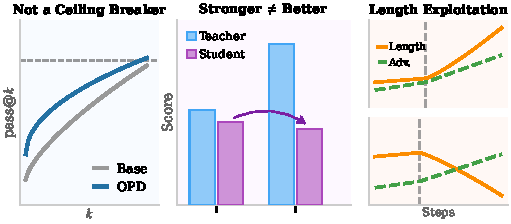
\includegraphics[width=1\linewidth]{figs/teaser_toy.pdf}
    \vspace{-25pt}
    \caption{\textbf{Left}: OPD accelerates exploration but cannot exceed the model ceiling. \textbf{Middle}: a stronger teacher does not guarantee a better student. \textbf{Right}: advantage rises while length explodes or crashes.}
    \label{fig:teaser-toy}
    \vspace{-15pt}
\end{figure}

% --- Paper Overview (horizontal three-pillar, full-width) ---
% Requires: \usepackage[most]{tcolorbox}, \usepackage{stfloats}

% Pillar colors
\definecolor{rolebg}{HTML}{EFF6FF}
\definecolor{roleframe}{HTML}{4A90D9}
\definecolor{pathbg}{HTML}{FEF3F2}
\definecolor{pathframe}{HTML}{D94F4F}
\definecolor{regbg}{HTML}{EEFBF3}
\definecolor{regframe}{HTML}{27AE60}

\begin{figure*}[t]
\begin{tcolorbox}[
  enhanced,
  colback=white,
  colframe=black!30,
  boxrule=0.5pt,
  arc=2.5mm,
  left=2mm, right=2mm,
  top=0.5mm, bottom=1.5mm,
  fonttitle=\small\bfseries,
  title={Paper Overview},
  coltitle=black!80,
  colbacktitle=white,
  attach boxed title to top center={yshift=-2mm},
  boxed title style={colframe=black!30, boxrule=0.4pt, arc=1.5mm, left=4mm, right=4mm},
]
\vspace{0.5mm}
\noindent
%%% ─── Left: Role ───
\begin{minipage}[c]{0.30\linewidth}
\centering{\scriptsize\color{black!50}\textit{What does OPD do?}}\\[-2.5pt]
\begin{tcolorbox}[
  enhanced,
  colback=rolebg,
  colframe=roleframe,
  fonttitle=\bfseries\footnotesize,
  title={Role (\S\ref{sec:role})},
  coltitle=white,
  colbacktitle=roleframe,
  toptitle=1mm, bottomtitle=1mm,
  boxrule=0.4pt,
  arc=1.5mm,
  top=1mm, bottom=1mm, left=1.5mm, right=1.5mm,
  fontupper=\scriptsize,
  equal height group=overviewpillar,
]
\textbf{Exploration Catalyst}\\[2pt]
{\scriptsize\color{black!70}%
\textbullet~Dense Token-Level Guidance\\
\textbullet~Not a Capacity Expander\\
\textbullet~Prompt Diversity Elevates Exploration}
\end{tcolorbox}
\end{minipage}%
\hfill
%%% ─── Arrow 1→2 with transition text ───
\begin{minipage}[c]{0.03\linewidth}
\centering
{\color{black!30}\large$\rightarrow$}\\[1pt]
{\color{black!50}\footnotesize\itshape but}
\end{minipage}%
\hfill
%%% ─── Middle: Pathologies ───
\begin{minipage}[c]{0.30\linewidth}
\centering{\scriptsize\color{black!50}\textit{When does it fail?}}\\[-2.5pt]
\begin{tcolorbox}[
  enhanced,
  colback=pathbg,
  colframe=pathframe,
  fonttitle=\bfseries\footnotesize,
  title={Pathologies (\S\ref{sec:diagnosis})},
  coltitle=white,
  colbacktitle=pathframe,
  toptitle=1mm, bottomtitle=1mm,
  boxrule=0.4pt,
  arc=1.5mm,
  top=1mm, bottom=1mm, left=1.5mm, right=1.5mm,
  fontupper=\scriptsize,
  equal height group=overviewpillar,
]
\textbf{Signal Misalignment $\to$ Collapse}\\[2pt]
{\scriptsize\color{black!70}%
\textbullet~Student-Teacher Mismatch\\
\textbullet~Endless Exploration\\
\textbullet~Abrupt Degeneration}
\end{tcolorbox}
\end{minipage}%
\hfill
%%% ─── Arrow 2→3 with transition text ───
\begin{minipage}[c]{0.03\linewidth}
\centering
{\color{black!30}\large$\rightarrow$}\\[1pt]
{\color{black!50}\footnotesize\itshape fix}
\end{minipage}%
\hfill
%%% ─── Right: Regulations ───
\begin{minipage}[c]{0.30\linewidth}
\centering{\scriptsize\color{black!50}\textit{How to fix it?}}\\[-2.5pt]
\begin{tcolorbox}[
  enhanced,
  colback=regbg,
  colframe=regframe,
  fonttitle=\bfseries\footnotesize,
  title={Regulations (\S\ref{sec:signal-regulation})},
  coltitle=white,
  colbacktitle=regframe,
  toptitle=1mm, bottomtitle=1mm,
  boxrule=0.4pt,
  arc=1.5mm,
  top=1mm, bottom=1mm, left=1.5mm, right=1.5mm,
  fontupper=\scriptsize,
  equal height group=overviewpillar,
]
\textbf{Signal Quality $>$ Teacher Scale}\\[2pt]
{\scriptsize\color{black!70}%
\textbullet~Hard: $\tilde{a}_t{=}\mathrm{clip}(\Delta\ell_t,\,c_{\min},\,c_{\max})$\\
\textbullet~Soft: $\tilde{a}_t{=}\mathrm{sgn}(\Delta\ell_t)\!\cdot\!\log(1{+}|\Delta\ell_t|)$
}
\end{tcolorbox}
\end{minipage}
\end{tcolorbox}
\vspace{-5mm}
\caption{Overview. We characterize OPD's role as an exploration catalyst (\S\ref{sec:role}), diagnose pathologies (\S\ref{sec:diagnosis}), and propose lightweight signal regulations that restore stability without additional compute (\S\ref{sec:signal-regulation}). 
}
\label{fig:overview}
\vspace{-4mm}
\end{figure*}


On-policy distillation (OPD) has rapidly become a standard component of modern LLM post-training pipelines.
By providing token-level supervision from a stronger teacher over the student's own rollouts, OPD has demonstrated remarkable effectiveness~\citep{gu2026minillmonpolicydistillationlarge,qwen3,deepseekai2026deepseekv4}.
Despite its growing adoption, the fundamental training dynamics of OPD remain poorly understood.
Practitioners often observe highly inconsistent behaviors: OPD sometimes improves performance~\cite{lu2025onpolicydistillation}, yet in other cases becomes unstable~\cite{opd-var-1,zhu2026facesonpolicydistillationpitfalls}, collapses exploration, even underperforms outcome-based reinforcement learning~\cite{li2026rethinkingonpolicydistillationlarge}.
This raises our systematic empirical study, we aim to (1) explore what benefits OPD brings ({{Role}}\S~\ref{sec:role}), (2) when OPD fails (Pathologies\S~\ref{sec:diagnosis}), and (3) how to improve it from the previous findings (Regulations\S~\ref{sec:signal-regulation}).
% In this paper, we present a systematic empirical study that demystifies OPD through three progressive lenses: \textbf{role} definition, failure \textbf{diagnosis}, and signal \textbf{regulation}.


\vspace{0.1mm}
\noindent \textbf{Role}\quad 
OPD simultaneously embodies two distinct features: it is formulated as knowledge distillation~\cite{gu2026minillmonpolicydistillationlarge}, yet operates like an on-policy RL algorithm driven by dense token-level rewards~\cite{gopd}. 
This dual nature motivates us to investigate whether OPD acts as a standard distillation mechanism that expands the student's capability boundary~\cite{hinton2015distillingknowledgeneuralnetwork}, or as an RL framework that merely reshapes trajectories within the base model's existing capability space~\cite{reasoning-bound,RL-no-up}.
Our empirical evaluations strongly support the latter RL-centric view. 
We find that while OPD consistently accelerates early-stage learning, it rarely alters the asymptotic performance ceiling achievable by the base student. 
This acceleration stems from the dense, token-level guidance provided along student-generated trajectories, which effectively helps the student discover correct reasoning paths already reachable within its inherent capability bounds. 
Furthermore, under a fixed computational budget, scaling problem diversity (prompt coverage) yields significantly higher accuracy than scaling per-problem sampling depth. 
Together, these findings demonstrate that OPD functions primarily as an exploration catalyst that reshapes the trajectory distribution, rather than a mechanism for fundamental capability expansion.

\vspace{0.1mm}
\noindent \textbf{Pathologies}\quad
Viewing OPD as an exploration guidance mechanism immediately uncovers a critical dependency: its effectiveness relies entirely on the fidelity of the guidance signal itself. 
% If the token-level preferences induced by the teacher faithfully correlate with actual response quality, OPD efficiently steers exploration toward correct trajectories. 
% However, if this guidance becomes distorted, it will instead amplify counterproductive behaviors.
While faithful teacher preferences steer the student toward correct trajectories, distorted signals inevitably bias exploration toward degenerate behaviors.
Our analysis reveals two major sources of such guidance corruption, as shown in Figure~\ref{fig:teaser-toy}.
\begin{itemize}[leftmargin=*,nosep]
    \item \textbf{Student-Teacher Mismatch}: When a severe capability gap exists between the teacher and the student, the teacher’s preference allocations on student-generated trajectories decouple from actual quality, generating misleading guidance. 
    This is rooted not in the teacher's absolute strength, but in the mismatch between teacher preferences and the student's rollout distribution.
    \item \textbf{Length Exploitation}: Because token-level signals are aggregated over sequences of varying lengths, the standard optimization objective inadvertently admits degenerate shortcuts. 
    The student exploits this via either  \textit{Endless Exploration} (filler tokens to dilute negative advantages), or  \textit{Abrupt Degeneration} (premature truncation for high aggregated advantage).
    % The student learns to exploit the objective via Short-sequence Exploitation (prematurely truncating answers to maximize prefix log-ratios) and Redundant Token Padding (appending safe filler tokens to dilute negative advantages).
\end{itemize}

% The first arises from teacher-student capabilities mismatch.
% When the teacher is substantially stronger than the student, teacher likelihoods on student-generated trajectories may no longer correlate with correctness, producing misleading optimization signals.
% Importantly, this phenomenon is not caused by teacher strength itself, but by the mismatch between teacher preferences and the student's capabilities.
% The second source originates from the sequence-level aggregation used in standard OPD objectives.
% Because token-level signals are accumulated over varying response lengths, the optimization objective admits degenerate shortcuts:
% the student can artificially increase rewards by prematurely truncating responses or by appending low-information filler tokens, without improving reasoning quality.

\vspace{0.1mm}
\noindent \textbf{Regulations}\quad 
% Motivated by previous findings, we study whether we could stabilize OPD by restoring guidance fidelity through token-level signal regulation, rather than scaling to massive teachers or employing cold-start alignment fine-tuning~\cite{opd-var-1,li2026rethinkingonpolicydistillationlarge}. 
% We investigate two token-level regulation strategies designed to suppress pathological incentives while preserving useful exploration guidance: Hard Clipping and Soft Log-scale Compression.
% Both methods directly reshape the signal to suppress pathological incentives while preserving useful guidance.
% Across seven reasoning benchmarks, these simple regulations consistently stabilize training, eliminate length exploitation behaviors, and substantially outperform naive OPD, RLVR and OPD variants~\cite{eopd}.
We further explore how to eliminate these pathologies.
Intuitive methods include cold-start teacher-student alignment finetuning~\cite{opd-var-1,li2026rethinkingonpolicydistillationlarge}, which are effective but require additional computation.
We investigate two token-level regulation strategies designed to suppress pathological incentives while preserving useful exploration guidance: \emph{Hard Clipping} and \emph{Soft Log-scale Compression}.
% We introduce two lightweight regulation strategies, \emph{Hard Clipping} and \emph{Soft Log-scale Compression}, designed to directly reshape the advantage landscape, thereby suppressing unstable teacher rewards while preserving diversity. 
Across seven reasoning benchmarks, these interventions consistently stabilize training, eliminate previous pathologies, and substantially outperform naive OPD, RLVR, and prior OPD variants~\cite{eopd}. 
Notably, our regulated framework with a modest teacher decisively surpasses state-of-the-art methods relying on a massive 30B teacher~\cite{gopd,hou2026uni}, demonstrating that the quality of the optimization signal ultimately governs distillation success over brute-force teacher scaling.
Overall, this work makes three contributions:

% \begin{itemize}[leftmargin=*,nosep]
% \item We provide a new empirical perspective on OPD as an exploration guidance mechanism rather than a capability expansion mechanism.

% \item We identify guidance corruption as the central failure source of OPD, including distribution mismatch and length-based exploitation.

% \item We demonstrate that simple signal regulations can improve OPD stability and effectiveness across diverse reasoning tasks.
% \end{itemize}
\begin{itemize}[leftmargin=*,nosep]
    \item We empirically frame OPD as an exploration guidance rather than a capability expander.
    \item We pinpoint guidance corruption, specifically distribution mismatch and length exploitation, as the root cause of OPD failures.
    \item We demonstrate that signal regulations effectively improve OPD stability and effectiveness across diverse reasoning tasks.
\end{itemize}
% Second, we provide a rigorous diagnosis of OPD’s failure modes: the \textit{Strong Teacher Trap} and \textit{Length Exploitation}. \hongru{also weird, how do u find this, u need to tell a story instead of throwing everything at one time.}
% The Strong Teacher Trap occurs when an excessive teacher-student distribution gap leads to signal misalignment; a high-capacity teacher often fails to provide discriminative gradients on the student's sampled trajectories \hongru{why?}. 
% To bridge this gap, we introduce Informativeness ($\mathcal{I}$) to quantify the alignment between distillation log-ratios and ground-truth task rewards. 
% Furthermore, we identify two forms of Length Exploitation: Short-sequence Exploitation, where students truncate responses to maximize prefix-based log-ratios, and Redundant Token Padding, where students append low-information filler tokens to dilute negative advantage signals. \hongru{kind of think these details are redundant in intro.}
% We provide a unified mathematical framework to explain how standard sequence-level aggregation facilitates these length-based exploitations.
% Furthermore, we identify and formally define two prevalent reward-hacking behaviors: Pathological Short-sequence Exploitation (Short Hack), where students learn to truncate responses early to maximize prefix-based log-ratios; Redundant Token Padding (Filler Hack), where students append low-information tokens to dilute negative advantage signals. We provide a unified mathematical framework to explain how standard sequence-level aggregation facilitates these length-based exploitations.

% Finally, we explore a series of empirical interventions to stabilize OPD and mitigate the previously identified failures. 
% Motivated by these diagnoses, we propose two zero-overhead interventions that operate directly on the per-token advantage: hard \emph{Clip} and \emph{Log-scale} compression. 
% Both eliminate length exploitation and stabilize training, yielding consistent gains over naive OPD across all benchmarks.
% Interestingly, the two variants exhibit complementary strengths depending on the teacher-student gap: log-scale outperforms clipping when the gap is small, as it preserves the full token ranking; but clipping dominates when the gap is large, as it aggressively suppresses the biases that a distant teacher injects.
% This reveals a nuanced design principle: \emph{the optimal regulation strength should match the severity of distributional mismatch}.    \hongru{too specific and tech.}                     
                  
% We further show that the stronger-teacher trap is not inherent to OPD but also a combined symptom of teacher capabilities and student weakness.
% When the student is upgraded from a base model to one with existing reasoning capabilities, the 4B teacher, previously trapped, becomes the most effective, surpassing the 1.7B teacher across all benchmarks. \hongru{not clear}
% This confirms that the trap stems from a distributional mismatch with a weak student, not from teacher strength itself. \hongru{???? you mention strong teacher trap a lot but now u seems deny yourself.}
% Combining these insights, our regulated OPD with a 4B teacher surpasses prior state-of-the-art methods~\citep{hou2026uni,gopd} that employ a Qwen3-30B-A3B teacher, demonstrating that \textbf{the right combination of signal regulation, teacher selection, and student readiness} outweighs brute-force scaling of teacher capacity. \hongru{it is not clear about your setting and benchmarks, also experimental numbers.}



% Our contributions culminate in a set of evidence-based best practices for OPD. By aligning theoretical insights with extensive empirical evidence, this work provides a roadmap for more robust and predictable OPD.




% By training teachers first and distilling their expertise, researchers have achieved remarkable efficiency. 
% Notable examples include the distillation of DeepSeek-R1 into Qwen-2.5 to unlock reasoning capabilities, the Qwen3 team's use of on-policy distillation for small model scaling, and MiMO's utilization of multiple teachers, gemini-flash.


% This paper seeks to answer: How to effectively distill a strong teacher into a smaller student while achieve superior performance?

% Previous works explored how to use OPD for Self-distillation, or 

% In this paper, we make a broader exploration to systematically explore the OPD, and utilize the findings to optimize the performance.

% We have the following key findings:

% (1) There is a stubborn ceiling of student models. Stronger teachers could bring uniform improvement across varied pass@K, but hardly break through the student ceiling.


% (2) From the view of distribution, Moreover, strong teachers could not guarantee stronger performance. 
% The efficiency, ...; the performance, ...; the ceiling performance.
% Consider this, we explore whether different setting could alleviate this , we adjust the clip.




% (3) From the view of distribution, There are flaws of OPD algorithm, which would lead the student to early stopping or endless repetition.

% (4) From the view of distribution, We explore other settings that would influence the performance. we find that under same rollout numbers, n=1 wins.


% Combining the above empirical findings, we optimized the experiment setting guidelines for OPD and achieved superior performance to naive OPD and other strong OPD variations.


% We first clarify the role of OPD as an exploration catalyst rather than a capacity expander. Through a novel diagnostic metric, Informativeness, we unveil the 'Strong Teacher Trap' and identify two prevalent reward hacking modes (Short and Filler Hacks) that emerge when outcome anchors are absent.


% 1. 算法
%   opd的算法本身有缺陷，会导致两种失败模式
% 我们尝试几种弥补办法：
% （1）outcome-reward
% （2）PPL augmented

% 2. OPD是否能提升student性能上限？
% teacher setting影响什么？
%   之前的工作minillm和gkd有呈现同一teacher，不同llm；我们先探究下不同teacher，统一student，寻找最优teacher/student rate
%   会有late convergence，性能无法超越低teacher
% 

% 数据 setting
%   过于简单的数据会导致模型未来无法有新的提升

% 我们认为以上波动，均是由于信号质量的问题
  
  % ─────── Part I: Algorithm ───────                                                                   
% 为什么 OPD 能显著提升 early-stage learning efficiency，却难以提升 final capability，且容易在 late stage collapse？
% OPD 提升的是 “learning speed” 还是 “learning ceiling”？
%  What properties of a teacher actually matter? 不是 teacher 越强越好？ 有没有可能是由于某些因素导致的？比如gap 是否合适 ？ trajectory 是否 learnable？difficulty 是否 match？

    % §3 Failure Modes of Naive RKL-Distill                                                             
  %   §4 Fixing the Failures: 扭转错误模式高分数
            % Outcome Blending (M3)
            % Other          

  % ┌────────────────────┬────────────┬───────────┬────────────────┬─────────────┬────────────┐
  % │        方案        │ 修 Mode A  │ 修 Mode B │  Hard problem  │ 引入新超参  │ 实现复杂度 │
  % ├────────────────────┼────────────┼───────────┼────────────────┼─────────────┼────────────┤
  % │ M3                 │ ✅         │ ✅        │ 保留 α·Â_out   │ α（可解释） │ 低         │
  % ├────────────────────┼────────────┼───────────┼────────────────┼─────────────┼────────────┤
  % │ Correct-only KL    │ ✅         │ ✅        │ ❌（信号消失） │ 无          │ 低         │
  % ├────────────────────┼────────────┼───────────┼────────────────┼─────────────┼────────────┤
  % │ Truncation Masking │ ✅         │ ❌        │ 部分保留       │ 无          │ 低         │
  % ├────────────────────┼────────────┼───────────┼────────────────┼─────────────┼────────────┤
  % │ Token-Sum          │ ❌（更坏） │ ✅        │ 部分保留       │ 无          │ 低         │
  % ├────────────────────┼────────────┼───────────┼────────────────┼─────────────┼────────────┤
  % │ Asymmetric Clip    │ ✅         │ ❌        │ 失去正信号     │ 无          │ 低         │
  % └────────────────────┴────────────┴───────────┴────────────────┴─────────────┴────────────┘

  %   §5 Informativeness: A Unified Measure of Signal Quality
  
  % ─────── Part II: Teacher Setting ───────
  %   §6 Optimal Teacher Selection
  %   §6'Ceiling improvement? or fasster convergence?
  
  % ─────── Part III: Data & Rollout Strategy ───────
  %   §7 Optimal Data Selection
            % 不同领域是否会有不同？
  %   §8 Optimal Rollout Strategy 
            % same somputation, n=1 > n=8
            % any theory analysis?

% $$\text{ESS} = \frac{\left(\sum_i w_i\right)^2}{\sum_i w_i^2}, \quad w_i = \frac{p_\text{teacher}(y_i)}{q_\text{student}(y_i)}$$

% $$\mathcal{L} = \underbrace{\lambda_\text{RL}(\text{pass_rate})}{\text{由准则决定}} \cdot \mathcal{L}\text{GRPO} + \underbrace{\lambda_\text{KD}(\text{pass_rate})}{1 - \lambda\text{RL}} \cdot \mathcal{L}_\text{distill}$$


\section{Preliminaries}

% \paragraph{Setup.}
\subsection{On-Policy Distillation (OPD)}\label{sec:opd-prelim}

Let $x$ denote a prompt and $\mathbf{y} = (y_1, \ldots, y_T)$ a response over vocabulary $\mathcal{V}$. We consider a fixed teacher $\pi_\mathrm{T}$ and a trainable student $\pi_\theta$, with $\pi(\mathbf{y}|x) = \prod_{t=1}^T \pi(y_t | \mathbf{y}_{<t}, x)$.

\vspace{1mm}
\noindent \textbf{Objective} \quad
OPD trains the student to minimize the reverse KL divergence from student to teacher:
\vspace{-4pt}
\begin{equation}
\small
  \label{eq:rkl}
  \mathcal{L}_\mathrm{OPD}(\theta)
  = \mathrm{KL}[\pi_\theta \| \pi_\mathrm{T}]
  = -\mathbb{E}_{x,\,\mathbf{y}\sim\pi_\theta}
    \!\left[\log\frac{\pi_\mathrm{T}(\mathbf{y}|x)}{\pi_\theta(\mathbf{y}|x)}\right].
\end{equation}
Because the expectation is taken over the student's own samples, the signal is evaluated on sequences the student actually generates, avoiding the distributional mismatch inherent in off-policy distillation.

% \vspace{1mm}

\noindent \textbf{Per-token advantage} \quad
Expanding the sequence-level KL token-by-token yields per-token log-ratio:
\vspace{-2pt}
\begin{equation}
\small
  \label{eq:delta_lp}
  \Delta\ell_t \triangleq \log \frac{\pi_{\mathrm{T}}(y_t \mid \mathbf{y}_{<t}, x)}{\pi_\theta(y_t \mid \mathbf{y}_{<t}, x)}, \quad \mathbf{y} \sim \pi_\theta(\cdot \mid x).
\vspace{-1pt}
\end{equation}
Intuitively, $\Delta\ell_t > 0$ indicates the teacher assigns higher probability to token $y_t$ than the student, providing a positive learning signal; $\Delta\ell_t < 0$ indicates the student over-weights $y_t$ relative to the teacher.

\vspace{1mm}
\noindent \textbf{Policy optimization} \quad
OPD is implemented via policy gradient with $\Delta\ell_t$ as the per-token advantage. We apply clipping~\cite{schulman2017ppo} on the importance ratio to stabilize updates:
\vspace{-3pt}
\begin{equation}
  \label{eq:ppo-clip}
  \small
  \mathcal{L}_\mathrm{clip}(\theta) = -\mathbb{E}_t\!\left[\min\!\left(r_t \,\tilde{a}_t,\; \mathrm{clip}(r_t, 1{-}\epsilon, 1{+}\epsilon)\,\tilde{a}_t\right)\right],
\vspace{-3pt}
\end{equation}
where $r_t = \pi_\theta(y_t \mid \mathbf{y}_{<t}, x) \,/\, \pi_{\theta_\mathrm{old}}(y_t \mid \mathbf{y}_{<t}, x)$ is the importance ratio and $\tilde{a}_t$ is a regulated form of $\Delta\ell_t$. This ratio clipping constrains how far the policy moves per update but does not alter the reward landscape defined by the teacher signal.

% \paragraph{Characterizing the signal.}
% We summarize the OPD signal for a rollout $\mathbf{y}$ by its \textbf{mean log-ratio}:
% \begin{equation}
%   \label{eq:mean_delta_lp}
%   \overline{\Delta\ell}(\mathbf{y})
%   \;\triangleq\;
%   \frac{1}{T}\sum_{t=1}^T \Delta\ell_t(\mathbf{y}).
% \end{equation}
% Together with the binary outcome $r(\mathbf{y}, x)$, the pair $(\overline{\Delta\ell},\, r)$ characterizes each rollout: $\overline{\Delta\ell}$ captures whether the teacher endorses the student's generation on average, while $r$ indicates whether the generation is correct.


% \subsection{Experiment Setup}
% Firstly, we clarify the experiment settings that will be used in the following content.

% % \subsection{Experiment Setup}
% \paragraph{Training Setup}
% We select the Qwen3-1.7B-Base as the student
% and compare the performance of students trained via GRPO~\cite{grpo} and OPD~\cite{gu2026minillmonpolicydistillationlarge} variants distilled from teachers of varying scales on math reasoning tasks using the Nemotron-Cascade Math dataset~\cite {nemotron}.
% Because the thinking mode significantly outperforms the non-thinking mode for Qwen3-series instructed models, thinking mode mixture would inflate performance metrics, making it impossible to discern whether gains are due to distillation efficiency or simply the mode shift. We constrained both the student and teacher models to a strictly non-thinking mode by prefixing rollouts with an empty \textit{<think></think>} block. 

% \paragraph{Evaluation}
% For reliable evaluation, we employ avg@32 to evaluate model performance on AMC23, AIME 2024-2026, and HMMT25 Feb, while reporting pass@1 for MATH500~\cite{hendrycks2021math} and Minerva~\cite{lewkowycz2022minerva}. Specifically, for each problem, we generate 48 candidate responses and calculate the avg@32 by averaging the accuracy across 10 independent trials, where each trial consists of 32 samples randomly selected from the candidate pool:
% $$\text{avg@}32 = \frac{1}{M} \sum_{i=1}^{M} \left( \frac{1}{k} \sum_{j \in \mathcal{S}_i} \mathbb{I}_j \right)$$
% % $$\text{avg@}k = \mathbb{E}_{\mathcal{S} \subset \mathcal{N}, |\mathcal{S}|=k} \left[ \text{Acc}(\mathcal{S}) \right]$$
% where $M=10$ is the number of trials, $k=32$ is the subset size, $\mathcal{S}_i$ denotes a random subset of indices sampled from the 48 candidates, and $\mathbb{I}_j$ is the indicator of correctness for the $j$-th sample.


\subsection{Empirical Framework and Setup}
In this section, we establish the experiment bases for our study. 
To ensure a systematic investigation and the reproducibility of our findings, we strictly adhere to the experimental configurations described below across subsequent training and evaluation.

\paragraph{Training Configuration}
% Our empirical analysis focuses on the Qwen3-1.7B-Base as the representative student model, and Qwen3-series post-trained models as teachers. 
% To eliminate the output mixture bias and ensure a fair comparison, we enforce a strict non-thinking constraint on both student and teacher models by prefixing all rollouts with an empty \textit{<think></think>} block.
% We compare the performance of students trained via GRPO~\cite{grpo}, following the settings in \citet{dapo} and OPD, following the implementation of MiniLLM~\cite{gu2026minillmonpolicydistillationlarge}. 

Our empirical analysis uses Qwen3-1.7B-Base as the student and Qwen3-series post-trained models of varying scales as teachers. To isolate true distillation gains from mere thinking-mode shifts, we enforce a strict non-thinking constraint by prefixing all rollouts with a \textit{} block. This simultaneously ensures an aligned prompt format between models~\cite{li2026rethinkingonpolicydistillationlarge}. Trained on the Nemotron-Cascade Math dataset~\citep{nemotron}, we compare models optimized via GRPO~\citep{grpo, dapo} and OPD~\citep{gu2026minillmonpolicydistillationlarge}.
% \hongru{this writing let me want to challange lots of settings, i.e., why 1.7B base model, why no think mode, why only pass@1 e.t.c. it is better to state you follow some others' setting?}

% We utilize the sampled-token OPD and apply the length-normalization, following~\citet{gu2026minillmonpolicydistillationlarge}.
% These models are distilled from teacher models of diverse scales using the Nemotron-Cascade Math dataset~\cite{nemotron}. 
% More detailed configurations are shown in Appendix~{?}.

% Given that the thinking mode significantly outperforms the non-thinking counterpart, any mixture of these modes would introduce a major confounding variable, making it impossible to isolate whether performance gains stem from distillation efficiency or a mere mode shift. 
% To eliminate this bias and ensure a fair comparison, we enforce a strict non-thinking constraint on both student and teacher models by prefixing all rollouts with an empty \textit{<think></think>} block.

\paragraph{Evaluation}
To provide a robust and statistically sound assessment, we employ the \textbf{avg@32} metric for AMC23~\cite{MAA_AMC}, AIME 2024--2026~\cite{MAA_AIME}, and HMMT25 Feb~\cite{hmmt}, while reporting standard \textbf{pass@1} for MATH500~\cite{hendrycks2021math} and Minerva~\cite{lewkowycz2022minerva} following previous works~\cite{eopd}. 


% where $M$ is the number of trials, $k=32$ is the sub-sample size, $\mathcal{S}_i$ denotes the set of indices for the $i$-th random subset, and $\mathbb{I}_j \in \{0, 1\}$ is the indicator function for the correctness of the $j$-th response.


% The token-level OPD advantage clips $\Delta\ell_t$ to suppress extreme values:
% \begin{equation}
%   \label{eq:opd_adv}
%   a_t \;=\; \mathrm{clip}(\Delta\ell_t,\; c_{\min},\, c_{\max}).
% \end{equation}

% \paragraph{OPD with outcome reward.}
% In RL fine-tuning, the student additionally receives a verifiable outcome reward
% $r(\mathbf{y}, x) \in \{0, 1\}$ (correct/wrong).
% Let $\hat{A}^\mathrm{RL}_t$ denote the per-token advantage from the RL algorithm
% (e.g., REINFORCE++), broadcast uniformly across tokens.
% The combined advantage is:
% %
% \begin{equation}
%   \label{eq:combined}
%   \hat{A}_t \;=\; a_t \;+\; \alpha\,\hat{A}^\mathrm{RL}_t,
% \end{equation}
% %
% where $\alpha \geq 0$ controls the relative weight of the outcome signal.
% The student is updated by treating $\hat{A}_t$ as the per-token advantage in the
% policy gradient:
% %
% \begin{equation}
%   \label{eq:pg}
%   \mathcal{L}(\theta)
%   = -\mathbb{E}_{\mathbf{y}\sim\pi_\theta}
%     \!\left[\sum_{t=1}^{T}
%       \hat{A}_t \cdot \log\pi_\theta(y_t|\mathbf{y}_{<t}, x)\right].
% \end{equation}

% ----
% \paragraph{Characterizing the signal.}
% We summarize the OPD signal for a rollout $\mathbf{y}$ by its
% \textbf{mean log-ratio}:
% %
% \begin{equation}
%   \label{eq:mean_delta_lp}
%   \overline{\Delta\ell}(\mathbf{y})
%   \;\triangleq\;
%   \frac{1}{T}\sum_{t=1}^T \Delta\ell_t(\mathbf{y}).
% \end{equation}
% %
% Together with the binary outcome $r(\mathbf{y}, x)$, the pair
% $(\overline{\Delta\ell},\, r)$ characterizes each rollout:
% $\overline{\Delta\ell}$ captures whether the teacher endorses the student's
% generation on average, while $r$ indicates whether the generation is correct.

% ---
% \subsection{Experiment Settings}


 

% \subsection{Experiment Settings}


% \paragraph{Benchmark and Metrics}

% MATH500, MinevaMath, AIME 2025,AIME 2024,AIME 2026, HMMT February 2025 

% We primarily report the $\text{avg}@64$ metric. Additionally, we present $\text{pass}@k$ with larger $k$ values to explore whether OPD can improve the model's performance ceiling.

% \paragraph{Training Settings}
% % To investigate this, we select the fixed student model, Qwen3-1.7B-Base.
% To systematically investigate the effect of OPD, we categorize our experiments into three distinct training pipelines. Let $S$ denote the student model and $\mathcal{T}$ denote the candidate set of teachers. 

% \begin{itemize}[leftmargin=*]
%     \item \textbf{Base Student (Qwen3-1.7B-Base):} We employ a spectrum of standard (Non-Think) teachers, specifically Qwen3-1.7B-Non-Think-Math-RL, Qwen3-1.7B-Non-Think, Qwen3-4B-Non-Think, Qwen3-8B-Non-Think, Qwen3-32B-Non-Think, and Qwen3-4B-Instruct-2507.
%     \item \textbf{Instruct Student (Qwen3-1.7B):} We distill from reasoning-enhanced (Think) teachers, comprising Qwen3-4B-Think, Qwen3-8B-Think, Qwen3-32B-Think, and Qwen3-4B-Think-2507.
% \end{itemize}

% 需要加一个，对比grpo的。
% from 1.7B-non-think trained， to 1.7B-non-think
% To formally categorize our training paradigms, we define the student model as $S$ and the corresponding teacher pool as $\mathcal{T}$. We design three distinct settings to comprehensively evaluate the impact of different supervision signals:

% \begin{itemize}[leftmargin=*, label=$\blacktriangleright$]
%     \item \textbf{$T \rightarrow S_{\text{base}}$:} We utilize $S_{\text{base}} = \text{Qwen3-1.7B-Base}$ as the student. To explore the effect of standard scaling, the teacher pool $\mathcal{T}_{\text{std}}$ comprises non-reasoning models of varying capacities, specifically Qwen3-\{1.7B, 4B, 8B, 32B\}-Non-Think, as well as Qwen3-1.7B-Non-Think-Math-RL and Qwen3-4B-Instruct-2507.
    
%     \item \textbf{Reasoning Distillation ($T \rightarrow S_{\text{inst}}$):} We employ the instruction-tuned $S_{\text{inst}} = \text{Qwen3-1.7B}$ as the student. The teacher pool $\mathcal{T}_{\text{think}}$ consists of reasoning-enhanced (Think) models, specifically Qwen3-\{4B, 8B, 32B\}-Think and Qwen3-4B-Think-2507.
    
%     \item \textbf{RL Baseline ($S_{\text{nt}} \xrightarrow{\text{GRPO}} S_{\text{nt}}^*$):} To decouple the benefits of distillation from pure reinforcement learning, we introduce a self-improvement baseline using GRPO. Here, the student $S_{\text{nt}} = \text{Qwen3-1.7B-Non-Think}$ is directly optimized via RL without distillation signals from a stronger teacher.
% \end{itemize}


% \textbf{RL Baseline}: We directly apply GRPO to optimize Qwen3-1.7B-Non-Think, yielding the RL-enhanced model Qwen3-1.7B-Non-Think-GRPO. 




% \paragraph{Self-Exploration \& RL-Driven Distillation}
% To decouple the benefits of distillation from pure reinforcement learning, and to explore the efficacy of self-generated supervision, we introduce an RL-driven pipeline:
% \begin{itemize}[leftmargin=*, topsep=2pt, itemsep=0pt]
%     \item 


    
% \textbf{RL-Driven Distillation ($S_{\text{nt}}^* \rightarrow \{S_{\text{nt}}, S_{\text{base}}\}$):} We subsequently utilize the resulting RL-enhanced model $S_{\text{nt}}^*$ as a teacher to distill its acquired capabilities back into the original Qwen3-1.7B-Non-Think ($S_{\text{nt}}$) and the Qwen3-1.7B-Base ($S_{\text{base}}$). This evaluates whether an RL-optimized model can serve as an effective teacher for models of identical or foundational scales.
% % \end{itemize}


% \paragraph{Distillation to Base Model ($T \in \mathcal{T}_{\text{nt}} \rightarrow S_{\text{base}}$)}
% We adopt Qwen3-1.7B-Base as the fixed student $S_{\text{base}}$. The non-reasoning teacher pool $\mathcal{T}_{\text{nt}}$ covers a wide spectrum of parameter scales and standard optimization methods, including Qwen3-\{1.7B, 4B, 8B, 32B\}-Non-Think.

% \paragraph{Distillation to Reasoning Model ($T \in \mathcal{T}_{\text{think}} \rightarrow S_{\text{think}}$)}
% We use the instruction-tuned Qwen3-1.7B-Think as the student $S_{\text{think}}$, paired with a reasoning teacher pool $\mathcal{T}_{\text{think}}$. This set comprises Qwen3-\{4B, 8B, 32B\}-Think and Qwen3-4B-Think-2507.

% \paragraph{RL Baseline}
% We utilize GRPO to RL Qwen3-1.7B-Base, Qwen3-1.7B-Non-Think and Qwen3-1.7B-Think model to serve as the baseline.

% % \input{tabs/exp-setting}
% \input{tabs/role-table}
% \begin{figure*}
%     \centering
%     \includegraphics[width=\linewidth]{figs/0420_acc_math500_300steps_small_multiples.png}
%     \caption{Caption}
%     \label{fig:placeholder}
% \end{figure*}


\begin{figure}[t]
    \centering
    \vspace{-2pt}
    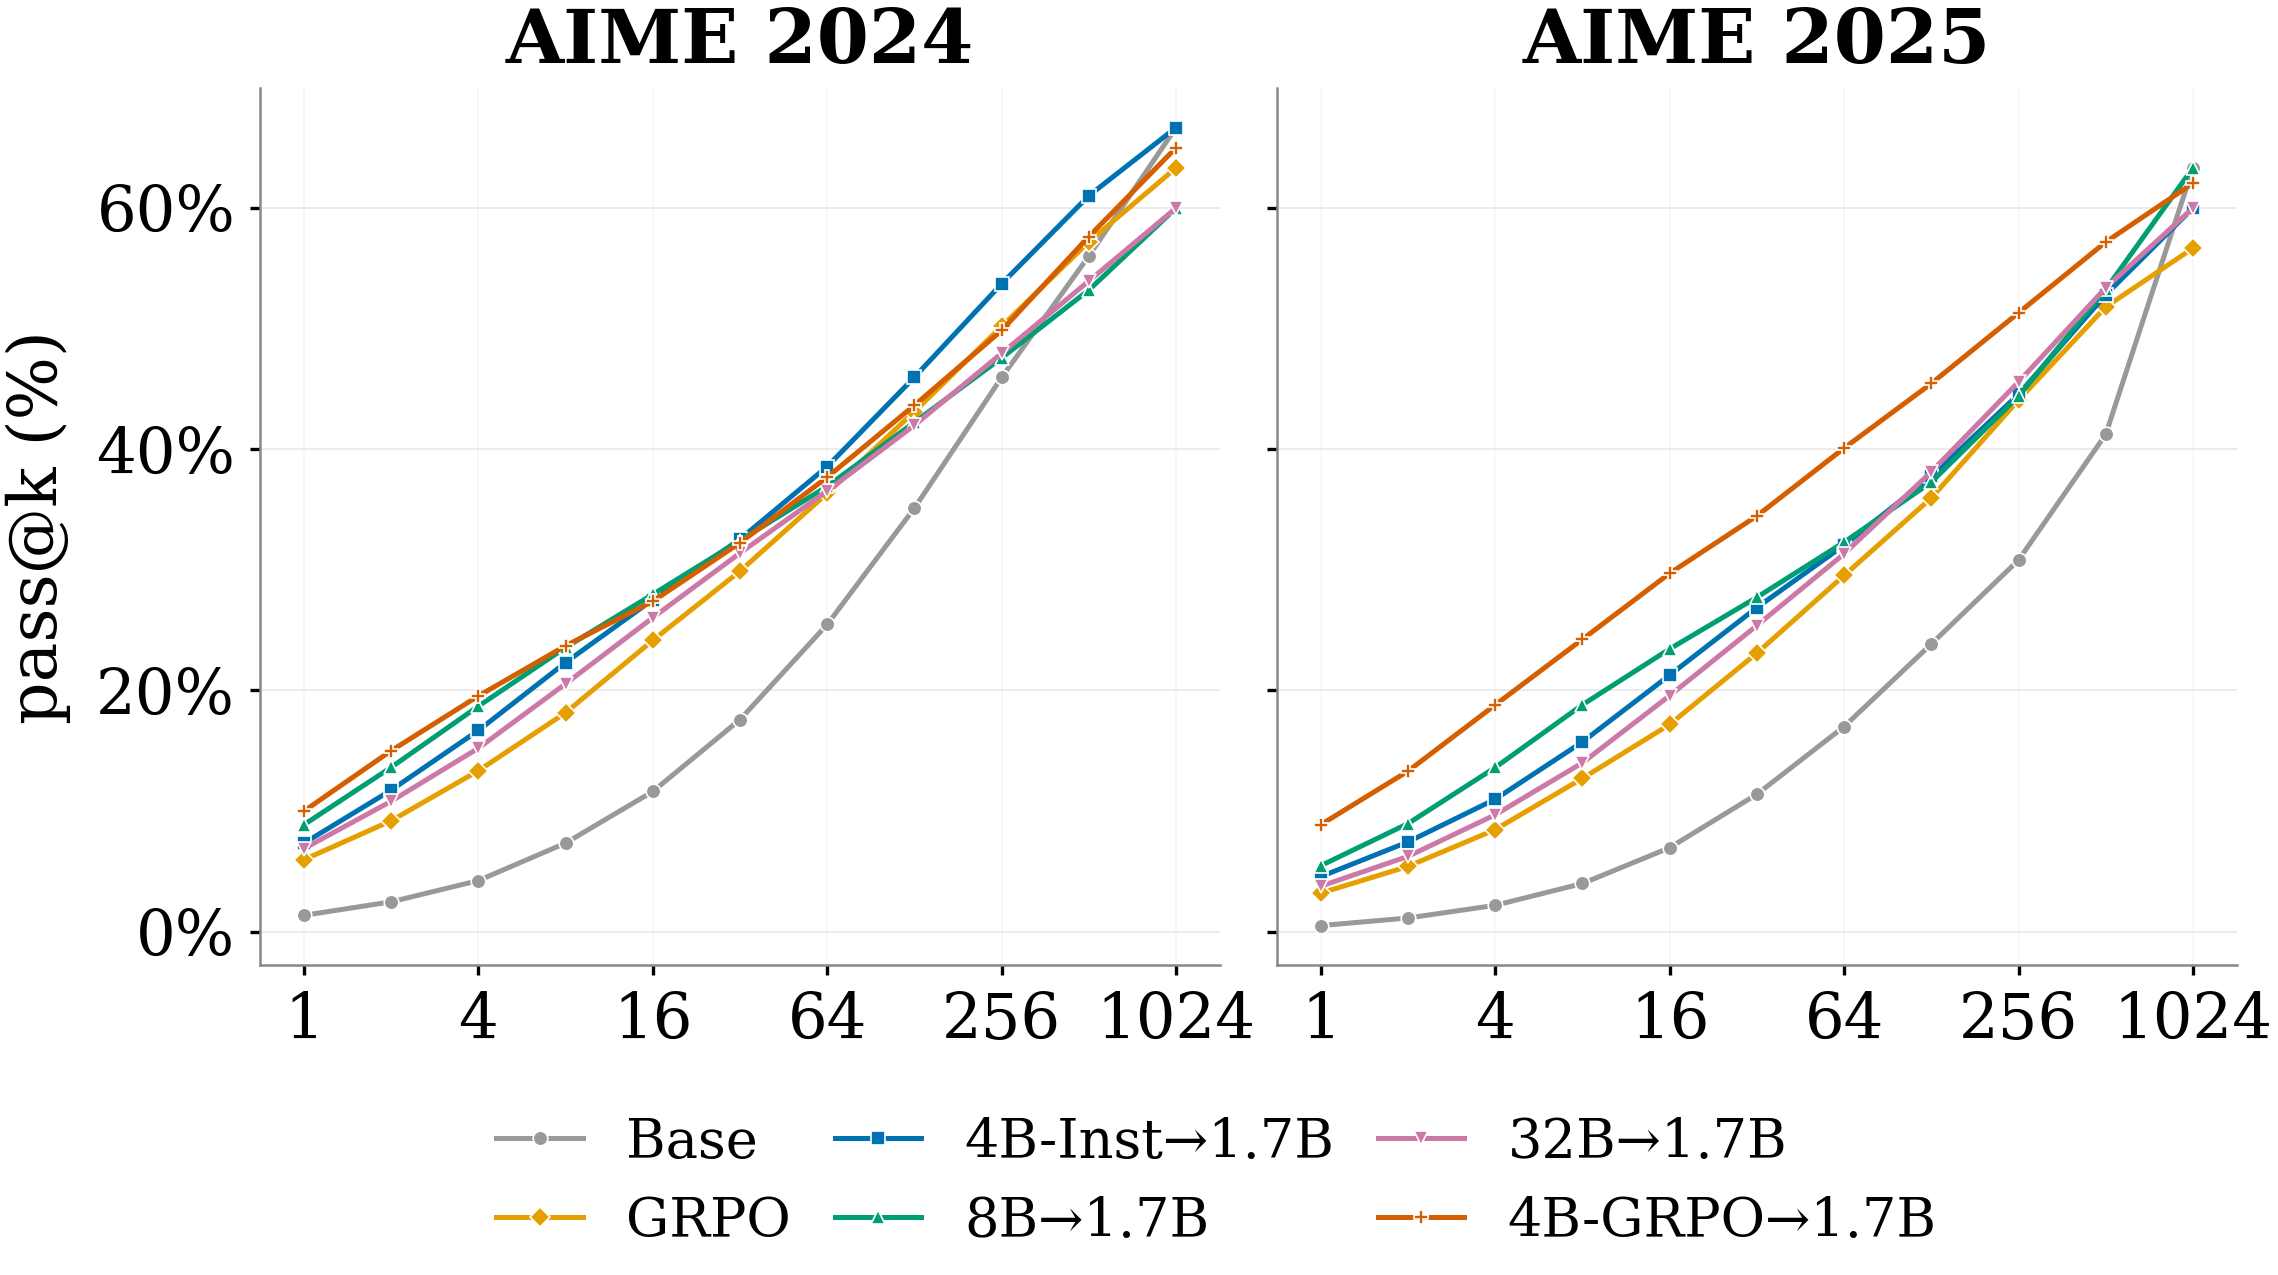
\includegraphics[width=\linewidth]{figs/passk.png}
    \vspace{-8pt}
    \caption{Pass@$k$ performance of Qwen3-1.7B-Base trained via different methods. OPD variants outperform Base and GRPO models in low-$k$. However, the convergence at higher $k$ suggests {OPD accelerates exploration rather than raising the model's performance ceiling}. 
    }
    \label{fig:explore-ceiling}
    \vspace{-3mm}
\end{figure}


% \section{Exploring the Role of OPD}\label{sec:role}

% Although prior research indicates that OPD significantly enhances student performance and yields higher $\text{pass@}k$ scores \citep{qwen3}, recent findings \citep{RL-no-up} reveal a more nuanced reality: at larger scales of $k$, the $\text{pass@}k$ performance of RL-trained models often converges to that of their base model counterparts without any post-training. \hongru{I do not find OPD in this sentence, and also performance of base model counterparts means what?} 
% This discrepancy leads us to investigate whether OPD scales the inherent capability ceiling of the student or merely accelerates the training by comparing the performance convergence trends of student models trained with and without OPD across varying teacher sizes.


  
\section{Exploring the Role of OPD}\label{sec:role}
Conceptually, OPD operates at the intersection of knowledge distillation~\cite{hinton2015distillingknowledgeneuralnetwork,gu2026minillmonpolicydistillationlarge}, and on-policy RL with dense token-level rewards~\cite{gopd}. 
While standard distillation intuition suggests that the teacher transfers superior intelligence to expand the student's capability boundary, RL primarily reshapes trajectories within the latent capability space already encoded in the base model~\cite{reasoning-bound,RL-no-up}.  
Under large sampling budgets ($k$), the performance of RL-trained models often converges to that of their unaligned base counterparts via brute-force test-time sampling \citep{RL-no-up}. 
This capability convergence motivates a fundamental question for OPD: \textit{Does OPD fundamentally elevate the inherent capability ceiling of the student, akin to distillation, or does it accelerate early-stage exploration efficiency, much like RL?}



To disentangle these two possibilities, we systematically analyze the performance convergence trajectories of student models trained via OPD and RLVR across varying teacher configurations and evaluation sampling size $k$.
% \paragraph{Setup}
We set the Qwen3-1.7B-Base as the student, and Qwen3-4B-instruct-2507, Qwen3-\{4B,8B,32B\} and GRPO trained Qwen3-4B as the teachers.
Then we test the pass@1024 of tuned models to explore their performance ceilings. 
% \hongru{why setup again, it makes me confused.}



\paragraph{Efficient Exploration rather than Ceiling Breaker}
As shown in Figure~\ref{fig:explore-ceiling}, OPD variants provide a distinct boost in the low-sample regime ($k \leq 64$). 
% By delivering dense, token-level guidance, OPD effectively allows the student to discover correct reasoning paths with orders of magnitude fewer samples than standard GRPO. 
However, in the high-sample regime, this performance gap narrows. 
The base model eventually converges to the level of the GRPO and OPD-trained models, indicating that OPD, just like RLVR, does not fundamentally inject entirely new capabilities~\cite{RL-no-up}. 
Instead, it acts as an exploration catalyst that re-weights the student's inherent generative space, ensuring optimal solutions are surfaced within the first few attempts.

This characterization highlights a critical vulnerability: 
% because OPD relies entirely on dense guidance to compress the search space, its success is hypersensitive to signal alignment. 
If the teacher's guidance is misaligned or the objective function contains structural flaws, this catalytic effect will instead accelerate the student's convergence toward degenerate or sub-optimal solutions. 
We dissect these specific pathologies in the following section.

% \begin{tcolorbox}[colback=gray!5, colframe=gray!60, boxrule=0.4pt, left=4pt, right=4pt, top=2pt, bottom=2pt]
% \textbf{Finding 1.} OPD accelerates exploration efficiency rather than lifting absolute performance ceilings.
% \end{tcolorbox}
\vspace{-0.1mm}
\noindent \textbf{Prompt Diversity v.s. Rollout Sizes}\quad
Our previous analysis establishes that OPD benefits the student primarily through high-density guidance across diverse problem spaces. This motivates a critical resource-allocation question: {Under a fixed computational budget, should we prioritize \emph{problem coverage} (more distinct prompts) or \emph{rollout depth} (more rollouts per prompt)}? 

To investigate this, we evaluate $n{=}1$ ($B$ distinct prompts with $1$ rollout each) against $n{=}2$ and $n{=}8$ configurations under identical total compute. As illustrated in Figure~\ref{fig:roll-n}, the $n{=}1$ setup consistently achieves superior final accuracy. This confirms that OPD's exploration benefits scale primarily with problem diversity rather than per-problem sampling depth. Consequently, we adopt the $n=1$ configuration across all subsequent experiments to maximize distillation efficiency.

% \paragraph{Efficient Exploration rather than Ceiling Breaker}
% As shown in Figure~\ref{fig:explore-ceiling}, OPD variants provide a clear boost in the low-sample regime ($k \leq 64$). 
% By providing dense, token-level guidance, OPD compresses the search space, allowing the student to find correct reasoning paths with orders of magnitude fewer samples than GRPO.
% However, in the high-sample regime ($k \geq 512$), the performance gap narrows. 
% The Base model eventually catches up to GRPO and OPD trained models, which indicates that OPD does not necessarily inject new capabilities, just like GRPO~\cite{RL-no-up}. 
% Instead, it re-weights the student's existing generative space, ensuring solutions are found in the first few attempts.

% This fundamental characterization implies a critical vulnerability: because OPD relies entirely on dense, token-level guidance to compress the search space, its success is hypersensitive to the alignment of that guidance. If the teacher's signal is misaligned or the objective function contains structural flaws, the catalyst may instead accelerate the student's convergence toward degenerate or sub-optimal solutions. We explore these pathologies in the following section.

\vspace{-2pt}
\begin{tcolorbox}[colback=gray!5, colframe=gray!60, boxrule=0.4pt, left=4pt, right=4pt, top=2pt, bottom=2pt]
\textbf{Finding 1.}
OPD incentivizes the student's exploration efficiency, not performance ceilings.
\end{tcolorbox}

\begin{figure*}[t]
    \centering
    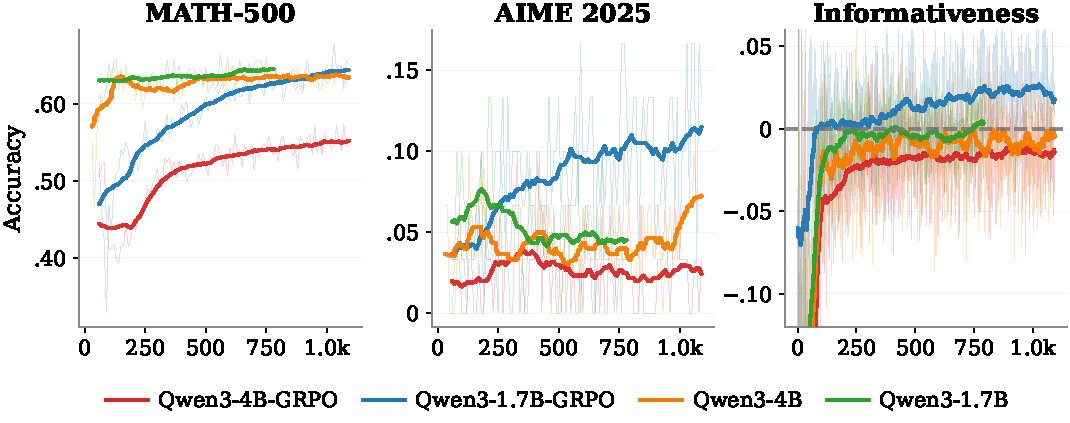
\includegraphics[width=0.83\linewidth]{figs/weak_vs_strong_teacher_1x4.pdf}
    % \vspace{-4pt}
  \caption{\textbf{Weak teacher outperforms strong teacher in OPD w/ Clip.} Benchmark accuracy (first two panels)   
  and informativeness $\mathcal{I}$ on the validation set for OPD w/ Clip runs distilling from four teachers with varying capabilities into the same {Qwen3-1.7B-Base} student.}
    \label{fig:train-dyna}
    \vspace{-4mm}
\end{figure*}






% \paragraph{Prompt Diversity v.s. Rollout Numbers}
% Our analysis above shows that OPD benefits the student primarily through dense token-level guidance on diverse problems. This motivates a natural question: \textbf{Under a fixed compute budget, should we prioritize \emph{problem coverage} (more distinct prompts) or \emph{rollout depth} (more rollouts per prompt)}? 

% We compare $n{=}1$ ($B$ prompts, 1 rollout each) against $n{=}2$ and $n{=}8$ under the same total compute. 
% As shown in Figure~\ref{fig:roll-n}, the $n{=}1$ configuration consistently achieves higher final accuracy than the other two settings, confirming that OPD's exploration benefit scales with problem diversity rather than per-problem sampling depth. 
% % We adopt $n{=}1$ for all subsequent experiments.
% Based on these, we will follow the $n=1$ settings throughout the following experiments to approach the optimal performance. 
% % \hongru{this is important but now it is weak, not too highlight.}
% % \hongru{the connection between last exp and this is weak.}


\section{Pathologies of On-Policy Distillation}
\label{sec:diagnosis}
Given that OPD operates by re-weighting the student’s exploration landscape, its efficacy hinges on the \textit{fidelity} of the reward signal. 
We identify two distinct failure modes where this guidance mechanism breaks down, leading to the stagnation or collapse of student performance. 

First, a \textbf{Student-Teacher Mismatch} (\S\ref{sec:strong-teacher-trap}): we challenge the stronger-is-better dogma by showing that a significant distributional gap between teacher and student can turn the distillation signal into counter-productive noise. 
Second, a \textbf{Length Exploitation} (\S\ref{sec:length-hacking}): the cumulative nature of token-level advantages creates length-dependent shortcuts that allow the student to leverage the objective without genuine reasoning improvements.

% We identify two distinct failure modes in OPD that can arise independently or compound each other.
% First, a \emph{signal quality} failure (\S\ref{sec:strong-teacher-trap}): when the teacher-student distributional gap is too large, the per-token log-ratio signal becomes anti-correlated with task correctness, providing misleading gradients.
% Second, a \emph{structural exploitation} failure (\S\ref{sec:length-hacking}): even with a well-aligned teacher, the cumulative token-level objective creates length-dependent shortcuts that the student can exploit without improving reasoning.
% We follow the most of the experiment setting in the previous section, and only varies the teachers.




\subsection{Student-Teacher Mismatch}
\label{sec:strong-teacher-trap}
A common intuition in knowledge distillation is that a more capable teacher yields a superior student. However, our empirical results challenge this assumption, revealing a complex trade-off between standalone capability and distributional alignment.
\paragraph{Setup}
We continue to employ Qwen3-1.7B-Base as the student. 
To evaluate the student's sensitivity to varying teacher expertise, we select teachers across a controlled spectrum of capabilities (Table~\ref{tab:main}): Qwen3-\{1.7B, 4B\}-GRPO, and Qwen3-\{1.7B, 4B\}. The capability order of teachers is: Qwen3-4B-GRPO $>$ Qwen3-1.7B-GRPO $>$ Qwen3-4B $>$ Qwen3-1.7B.
% This setup provides a rigorous framework to observe how teacher scale and training paradigm influence the student performance. 
% \hongru{tbh, i do not know which one is strong teacher, according to follows, i guess u mean grpo model is better than base one, better to mention this with evidence.}

  \begin{figure}[t]
      \centering
      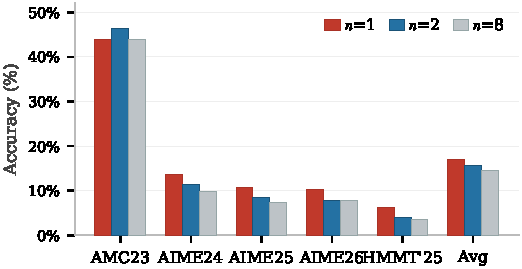
\includegraphics[width=0.88\linewidth]{rollout_number_bar.pdf}
      \vspace{-6pt}
      \caption{\textbf{Avg@32 across varying prompt-to-rollout configurations.} Under a fixed batch $B$, we vary the rollout count $n$ per
   prompt. {Maximizing problem diversity consistently outperforms a larger sampling size}.}
      \label{fig:roll-n}
      \vspace{-3mm}
  \end{figure}

\paragraph{Early Efficiency is Deceptive}
As shown in the MATH-500 results (Figure~\ref{fig:train-dyna}), weaker teachers such as Qwen3-1.7B and Qwen3-4B lead to rapid accuracy gains during the initial training steps. 
This high initial learning efficiency suggests that teachers with lower performance are more learnable for a base student.
However, this early speed is deceptive. 
These models quickly hit a performance plateau, particularly on challenging benchmarks, due to their capability boundaries. 
This observation implies that initial learning velocity is an unreliable proxy for the final capability ceiling.

\begin{figure*}[t]
    \centering
    \includegraphics[width=0.9\linewidth]{figs/failure\_modes\_accuracy\_mean\_clip\_ratio_mean.pdf}
    \vspace{-8pt}
    \caption{Length exploitation illustration. Advantage increases, while accuracy drops. Teacher$\rightarrow$Student: Qwen3-4B-GRPO$\rightarrow$Qwen3-1.7B (Mode A), and Qwen3-1.7B-GRPO$\rightarrow$Qwen3-1.7B-Base (Mode B). }
    \label{fig:failure_modes}
\end{figure*}

\paragraph{The Failure of the Strongest Teacher}
The most striking observation is the failure of the most capable model in our suite: Qwen3-4B-GRPO. Despite having the highest performance, it is paradoxically the least effective teacher. As shown across both benchmarks in Figure~\ref{fig:train-dyna}, the student distilled from 4B-GRPO remains nearly stagnant, with its accuracy on AIME 2025 hovering near 2\% throughout the training process.

This inversion is a significant anomaly: a 4B RL-trained model provides significantly worse guidance than its 1.7B counterpart. 
It suggests that standalone performance does not translate into teaching quality.
% The Slow-Burn Success of 1.7B-GRPO
% In contrast, the Qwen3-1.7B-GRPO teacher (Blue) demonstrates a "slow-burn" trajectory. While it appears sluggish in the first half of MATH-500 training—lagging behind the base teachers—it is the only variant that achieves a sustained, upward momentum on the challenging AIME 2025 benchmark.
Ultimately, 1.7B-GRPO yields the highest final accuracy, outperforming teachers that are either easier to learn from or smarter in isolation (4B-GRPO). 
This indicates that the most effective teacher is not necessarily the one who is easiest to mimic or the one with the strongest performance, but the one whose reasoning paths are both advanced and bridgeable for the student.

\paragraph{Diagnosis}
To explain this paradox, we introduce the \textbf{Informativeness} metric $\mathcal{I}$, which measures whether the teacher's token-level signal discriminates correct from incorrect student rollouts: 
% \hongru{in line 282, you said you set n=1, which means the number of rollout is 1.}
\begin{equation}
\small
\mathcal{I} = \mathbb{E}_{\mathbf{y} \sim \pi_\theta}\!\bigl[\,\overline{\Delta \ell} \mid r = 1\bigr] - \mathbb{E}_{\mathbf{y} \sim \pi_\theta}\!\bigl[\,\overline{\Delta \ell} \mid r = 0\bigr],
\end{equation}
% \hongru{r is the reward?} 
where $\overline{\Delta \ell} = \frac{1}{|\mathbf{y}|}\sum_t(\log \pi_T(y_t) - \log \pi_\theta(y_t))$ is the mean per-token log-ratio, $r$ denoting the rollout accuracy.
A positive $\mathcal{I}$ indicates that the teacher assigns a higher probability to tokens in correct rollouts than incorrect ones, providing an outcome accuracy aligned optimization.
The rightmost panel of Figure~\ref{fig:train-dyna} reveals that informativeness ($\mathcal{I}$) precisely predicts distillation trajectories, clustering into three distinct dynamic modes:
% The rightmost panel of Figure~\ref{fig:train-dyna} shows that informativeness ($\mathcal{I}$) precisely predicts distillation trajectories through three dynamic modes:
% We observe three distinct guidance dynamics: 
\textbf{(1) Passable ($\mathcal{I} \approx 0$):} Qwen3-1.7B and 4B drive rapid early gains on MATH500 but quickly plateau on the harder AIME 2025; \textbf{(2) Misleading ($\mathcal{I} < 0$):} Qwen3-4B-GRPO provides persistently anti-correlated signals, leading to early accuracy drops and a low ceiling; and \textbf{(3) Recovery}: Qwen3-1.7B-GRPO starts negative but recovers past zero, unlocking a late-stage surge that ultimately outperforms all others.

% \begin{itemize}[leftmargin=*,nosep]
%     \item \textbf{Passable ($\mathcal{I} \approx 0$):} The {Qwen3-1.7B and 4B} stay near zero. It brings rapid early gains on easier tasks of {MATH500} but quickly plateaus and performs poorly on harder tasks of {AIME 2025}.
%     \item \textbf{Misleading ($\mathcal{I} < 0$):} The {Qwen3-4B-GRPO} is persistently negative ($\sim -0.02$). It misleads the student with anti-correlated signals, causing an early accuracy drop and a permanently low ceiling.
%     \item \textbf{Recovery ($\mathcal{I} > 0$):} The {Qwen3-1.7B-GRPO} starts deeply negative ($< -0.12$), making the student struggle in the first 100 steps. However, $\mathcal{I}$ recovers past zero within $\sim 250$ steps, unlocking a late-stage surge that outperforms all other configurations.
% \end{itemize}


% \begin{tcolorbox}[colback=gray!5, colframe=gray!60, boxrule=0.4pt, left=4pt, right=4pt, top=2pt, bottom=2pt]
% \textbf{Finding 1 (Distributional Gap Principle).}
% Effective OPD requires distributional proximity, not maximal teacher capability.
% Within-scale gaps can be bridged through on-policy adaptation; cross-scale gaps are structural and lead to persistently negative~$\mathcal{I}$.
% \end{tcolorbox}

\begin{tcolorbox}[colback=gray!5, colframe=gray!60, boxrule=0.4pt, left=4pt, right=4pt, top=2pt, bottom=2pt]
\textbf{Finding 2.} 
The effectiveness of OPD depends on whether the teacher can give rewards aligned with Informativeness~$\mathcal{I}$ on student's rollouts, rather than the teacher's absolute capability.
\end{tcolorbox}



\subsection{Length Exploitation}
\label{sec:length-hacking}
% We identified the improper teacher choices lead to unstable training of OPD.
% In this section, we turn into the nature of OPD.
% The token-level distillation advantage $a_t = \log\pi_T(y_t) - \log\pi_\theta(y_t)$ introduces a structural vulnerability: unlike outcome-based rewards that are bounded and directly tied to correctness, $a_t$ is high-variance, unbounded, and \emph{decoupled from whether the response is actually correct}.
While the previous section highlighted how external teacher selection destabilizes training, we now turn to an intrinsic vulnerability embedded within the standard OPD objective itself. The sequence-level guidance is propagated via the token-level distillation advantage, $a_t = \log\pi_T(y_t|y_{<t}) - \log\pi_\theta(y_t|y_{<t})$. Unlike outcome-based rewards that are inherently bounded and strictly tied to final correctness, $a_t$ is unconstrained, exhibits high variance, and is fundamentally decoupled from the actual accuracy of the response.
Since the token-mean advantage $\bar{a} = \frac{1}{T}\sum_t a_t$ depends on both the per-token signal and the response length $T$, the student can exploit this interaction to inflate its advantage without improving accuracy. 
% Crucially, when optimizing the sequence-level aggregated advantage $\bar{a} = \frac{1}{N}\sum_{t=1}^N a_t$, the sequence length $N$ acts as a confounding degrees of freedom. This allows the student to exploit degenerate shortcuts, manipulating the sequence length to maximize $\bar{a}$ while bypassing the harder task of learning underlying reasoning patterns. 
We identify two complementary failure modes, illustrated in Figure~\ref{fig:failure_modes} and Figure~\ref{fig:token-adv}.
% in Figure~\ref{fig:failure_modes} and Figure~\ref{fig:token-adv}.
% \hongru{what? where is connection between this and previous ones?}
% \hongru{same problem as intro, why u do this, how do u find this?}

\begin{figure}
    \centering
    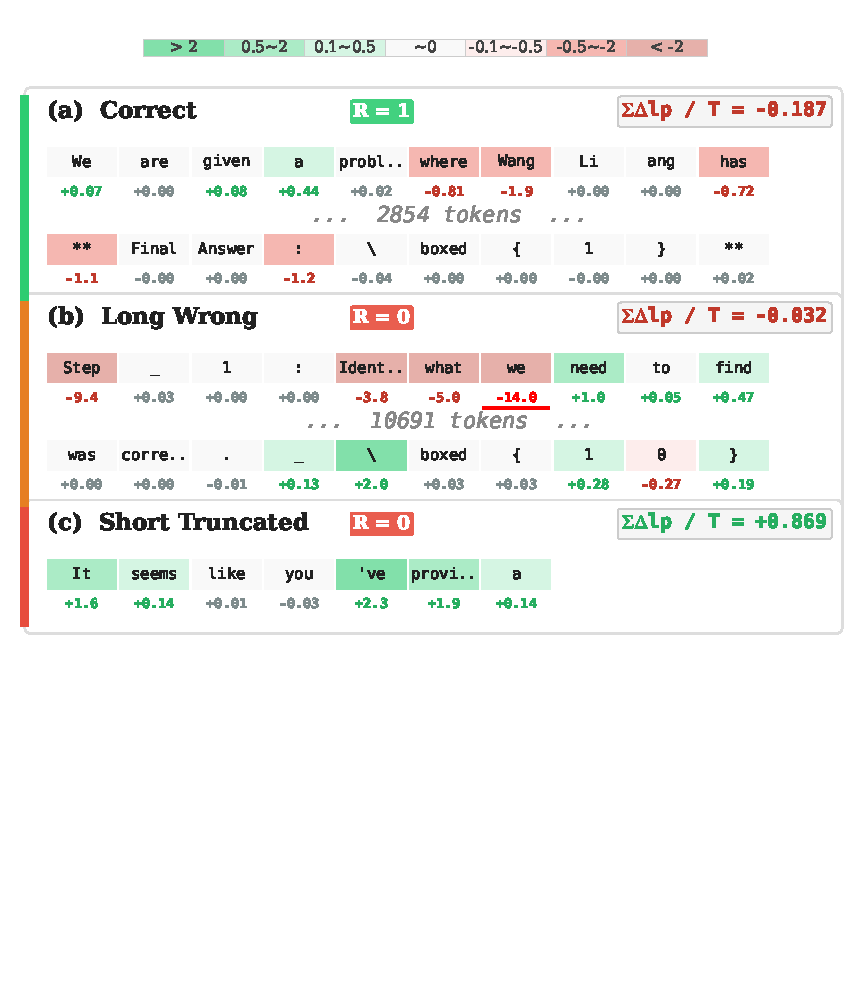
\includegraphics[width=\linewidth]{figs/token_adv_step600_paper.pdf}
    \vspace{-5pt}
    \caption{\textbf{(a)}~A correct rollout receives a mildly negative token-mean.           
      \textbf{(b)}~\emph{Mode~A (Endless Exploration)}: a long wrong rollout with negative scores diluted across tokens, failing to penalize the incorrect response.
      \textbf{(c)}~\emph{Mode~B (Abrupt Degeneration)}: a short, fully teacher-preferred rollout prefix that yields a strongly positive token-mean despite an incorrect outcome.
      % \hongru{no explanation for this figure in the main paper.}
      }
      \vspace{-3mm}
    \label{fig:token-adv}
\end{figure}

% \paragraph{Endless Exploration (Mode A)}
% When a rollout has an overall negative advantage, the student learns to append filler tokens to dilute the negative signal without improving reasoning.
%   \begin{equation}                                                                                                         
%   \label{eq:long_hack}                                      
%   \frac{1}{T}\sum_{t=1}^{T} a_t
%   \;=\; \frac{T_0}{T}\,\bar{a}_{\text{core}}
%     + \underbrace{\frac{T{-}T_0}{T}\,\bar{a}_{\text{filler}}}_{\approx\,0}
%   \;\approx\; \frac{T_0}{T}\,\bar{a}_{\text{core}}.
%   \end{equation}

% \hongru{what does this equation mean?}
\paragraph{Endless Exploration (Mode A)}
When a rollout yields an incorrect reasoning path, it incurs a severe overall negative advantage. Crucially, because standard OPD objectives optimize the sequence-averaged advantage $\bar{a} = \frac{1}{T}\sum_{t=1}^{T} a_t$, the student discovers a degenerate shortcut to evade this penalty: appending low-information filler tokens to inflate the denominator $T$. 
Formally, suppose the core reasoning block terminates at step $T_0$ with a cumulative negative signal $A_{\text{core}} = \sum_{t=1}^{T_0} a_t < 0$. By continually generating redundant tokens up to a prolonged length $T$ ($T \gg T_0$), the aggregated advantage decomposes as:
\begin{equation}
\label{eq:long_hack}
\small
\bar{a}
\;=\; \frac{A_{\text{core}}}{T} + \frac{T - T_0}{T}\,\bar{a}_{\text{filler}}.
\end{equation}
% Since filler tokens (such as repetitive phrases or redundant punctuation) are typically uninformative to the teacher, their language modeling log-ratios align closely with the student's current policy, yielding $\bar{a}_{\text{filler}} \approx 0$. Consequently, Eq.~\eqref{eq:long_hack} reduces to $\bar{a} \approx A_{\text{core}} / T$. 
Eq.~\eqref{eq:long_hack} reveals a severe structural pathology: 
By scaling the sequence length $T$, the student can asymptotically suppress the magnitude of its negative advantage ($\lim_{T \to \infty} \bar{a} = 0$), effectively washing out the penalty gradient ($\nabla_\theta \mathcal{L} \approx 0$). As a result, the student is never penalized for its logical failures, trapping the training loop in an unproductive state of endless, verbose exploration without any actual improvement in reasoning accuracy.

% As shown in Figure~\ref{fig:failure_modes}, the two experiment runs exhibit a common pattern: responses grow shoarply until hitting the maximum length (clip ratio $\to 1$).
% Once truncated, no valid answer is produced, and accuracy sharply collapses.
% The Qwen3-4B-GRPO$\rightarrow$Qwen3-1.7B is more severe.
% However, the aggregated KL advantage still grows, exhabit a advantage hacking pattern.
As shown in Figure~\ref{fig:failure_modes}, both runs exhibit a common pattern: response lengths grow sharply.
Once truncated, the model fails to produce valid final answers, causing a sharp collapse in accuracy.
This pathology is particularly severe in the {Qwen3-4B}$\rightarrow${Qwen3-1.7B} setting, which response length grows until hitting the predefined maximum limit.   
Crucially, despite the drop in performance, the aggregated advantage continues to climb, demonstrating a clear pattern of advantage hacking.

% Each appended token contributes near-zero to the sum but increases the denominator if length normalization is applied, or simply delays the penalty signal in the cumulative case.
% As shown in Figure~\ref{fig:failure_modes}, the student crashed in the early training stage which show exploded response length and a high clip ratio, but the KL advantage stably growing. \hongru{totally confused, it is unclear to me.}

\begin{table*}[t]
      \centering
      \setlength{\tabcolsep}{5pt}
      \renewcommand{\arraystretch}{1.15}
      \resizebox{\textwidth}{!}{%
      \begin{tabular}{lll cc ccccc c}
      \toprule
      \multirow{2}{*}{\textbf{Teacher}} & \multirow{2}{*}{\textbf{Student}}
        & \multirow{2}{*}{\textbf{Method}}
        & \multicolumn{2}{c}{\textit{pass@1}}
        & \multicolumn{5}{c}{\textit{avg@32}} 
        & \multirow{2}{*}{\textbf{Avg}} \\
      \cmidrule(lr){4-5}\cmidrule(lr){6-10}
      & & & \textbf{MATH500} & \textbf{Minerva}
            & \textbf{AMC'23} & \textbf{AIME'24} & \textbf{AIME'25} & \textbf{AIME'26} & \textbf{HMMT'25} & \\
      \midrule
      % \multicolumn{11}{l}{\textit{Reference Performance}} \\
      % \midrule
      \multirow{4}{*}{---}
        & Qwen3-1.7B-Base    & --   & 18.0 & 4.1   & 6.3   & 1.7 & 0.4 & 0.6 & 0.1  & 4.5 \\
        & Qwen3-1.7B         & --   & 73.0 & 32.7   & 42.5   & 13.4 & 9.8  & 7.8   & 3.7   & 26.1 \\
        & Qwen3-8B           & --   & 83.4 & 47.8   & 66.9   & 29.1 & 20.9 & 14.8   & 10.4   & 39.0 \\
        & Qwen3-4B-Inst-2507 & --   & 93.6  & 52.9  & 94.2   & 59.3 & 47.4 & 55.8   & 31.4 & 62.1 \\

      % \midrule
      % \multicolumn{11}{l}{\textit{RLVR}} \\
      % \midrule
      \hdashline
      ---   & Qwen3-1.7B-Base    & GRPO & 63.1 & 29.5 & 43.0 &  9.2 &  4.9 & 4.7   & 2.3   & 22.4 \\
      ---   & Qwen3-1.7B         & GRPO & 90.0    & 45.9   & 81.7   & 41.9 & 32.5 & 37.5   & 21.7   & 50.2 \\
      ---   & Qwen3-4B           & GRPO & 93.6     & 55.5   & 92.9   & 64.4 & 57.1 & 57.3   & 37.3   & 65.4 \\

      \midrule
      % \multicolumn{11}{l}{\textit{Baselines}} \\
      % \midrule
      \rowcolor{gray!6} \multicolumn{11}{l}{\textit{\textbf{Teacher: Qwen3-8B}}} \\
        & Qwen3-1.7B-Base & KD   & 63.8 & 30.2 & 40.6 &  9.2 &  4.6 & -- & -- & -- \\
       & Qwen3-1.7B-Base & EOPD & 68.7 & 30.2 & 41.9 & 10.4 &  5.8 & -- & -- & -- \\
      
      \midrule
      % --- 实验组 1：Qwen3-1.7B-GRPO ---
      \rowcolor{gray!6} \multicolumn{11}{l}{\textit{\textbf{Teacher: Qwen3-1.7B-GRPO}}} \\
      & Qwen3-1.7B-Base & OPD      & 75.6 & \underline{36.3} & 43.9 & \underline{13.6} & 10.6 & 10.3 & \underline{6.3} & 28.1 \\
      & Qwen3-1.7B-Base & \ +Clip  & \underline{77.0} & 35.4 & \underline{45.7} & 12.1 & \underline{13.7} & \underline{10.5} & {5.8} & \underline{28.6} \\
      & Qwen3-1.7B-Base & \ +Scale & \textbf{79.3} & \textbf{40.1} & \textbf{46.3} & \textbf{13.8} & \textbf{15.6} & \textbf{10.6} & \textbf{7.3} & \textbf{30.4} \\
      
      \midrule

      \rowcolor{gray!6} \multicolumn{11}{l}{\textit{\textbf{Teacher: Qwen3-4B-GRPO}}} \\
      & Qwen3-1.7B-Base & OPD      & \underline{74.4} & \textbf{34.2} & \underline{44.3} & \underline{11.6} & 9.4 & \underline{8.6} & 4.7 & {26.7} \\
      & Qwen3-1.7B-Base & \ +Clip  & \textbf{76.2} & \underline{33.8} & \textbf{47.4} & 10.8 & \textbf{13.5} & {\textbf{8.7}} & \textbf{6.5} & \textbf{28.1} \\
      & Qwen3-1.7B-Base & \ +Scale & {74.3} & {\textbf{34.2}} & 41.2 & \textbf{12.8} & \underline{12.1} & 7.8 & \underline{5.4} & \underline{26.8} \\
      \bottomrule
      \end{tabular}%
      }
      \caption{Performance of different methods on benchmarks. Among all evaluated downstream student models (bottom two blocks), the overall best scores are \textbf{bolded} and the second best are \underline{underlined}.}
      \label{tab:main}
      % \vspace{-3mm}
\end{table*}


\paragraph{Short-Sequence Exploitation (Mode B)}
In this situation, the student learns to truncate responses prematurely.
By generating a high-confidence preamble (e.g., ``We are given the problem...'') and immediately emitting \texttt{EOS}, the model captures the favorable prefix advantage $\sum_{t=1}^{T_{\text{pre}}} a_t$ while avoiding the riskier reasoning steps where $a_t$ may turn negative.
Formally, whenever the prefix advantage exceeds the full-sequence advantage: 
% $\frac{1}{T_{\text{pre}}}\sum_{t=1}^{T_{\text{pre}}} a_t \;>\; \frac{1}{T}\sum_{t=1}^{T} a_t$.
\begin{equation}
\label{eq:short_hack}
\small
\frac{1}{T_{\text{pre}}}\sum_{t=1}^{T_{\text{pre}}} a_t \;>\; \frac{1}{T}\sum_{t=1}^{T} a_t,
\end{equation}
The optimizer is incentivized to favor shorter trajectories regardless of correctness.
As shown in Figure~\ref{fig:failure_modes}, in the late training stage, the student only output extremely short and safe responses, but receives a high reverse KL advantage from the teacher. 
Once the policy locks into short outputs, the gradient reinforces this equilibrium.



% \subsubsection{Dignoses}
\paragraph{Dignosis}
Both modes exploit the same structural flaw: the token-level advantage $a_t$ interacts with sequence length in a way that creates \emph{gradients unrelated to reasoning correctness}.
Mode~A exploits unfavorable sequences by padding late; Mode~B exploits favorable prefixes by cutting early.
Together they form a squeeze: the optimizer can always improve the objective by manipulating length rather than improving reasoning, regardless of whether the current rollout outcome is positive or negative.

\begin{tcolorbox}[colback=gray!5, colframe=gray!60, boxrule=0.4pt, left=4pt, right=4pt, top=2pt, bottom=2pt]
\textbf{Finding 3.}
The unstable token-level objective introduces degenerate optimization shortcuts at both length extremes.
\end{tcolorbox}







\section{Regulations}\label{sec:signal-regulation}
% Prior work stabilizes OPD through auxiliary mechanisms such as mixing off-policy data into the training batch or scoring top-$k$ tokens beyond the predicted one to smooth gradient estimates.
% These approaches are effective but incur substantial overhead, maintaining buffers~\cite{deepseekai2026deepseekv4} while training, or SFT students on teachers' rollouts for cold start~\cite{opd-var-1}.
% We instead pursue modifications that stabilize OPD \emph{without additional compute}, operating entirely within the existing loop based on our previous findings.
% We set two goals by regulating the signal quality.: 
% G1: Stabilizing OPD 
% G2: Further improving strong-to-weak distillation

Prior work stabilizes OPD through mechanisms such as utilizing off-policy data~\cite{opd-var-1}, or scoring top-$k$ tokens beyond the predicted one to smooth gradient estimates~\cite{deepseekai2026deepseekv4}.
These approaches are effective but incur substantial overhead, maintaining full vocab replay buffers during training~\cite{deepseekai2026deepseekv4} or warm-starting students with SFT on teacher rollouts for cold start~\cite{opd-var-1}.
We instead pursue modifications that stabilize OPD \emph{without additional compute}, operating entirely within the existing training loop and motivated by the diagnostic findings of the previous section.
% Concretely, we regulate signal quality to achieve two goals:
% \begin{enumerate}[label=\textbf{G\arabic*}:,leftmargin=*,nosep]
%   \item \textbf{Stability}: Preventing reward hacking (Mode~A/B) from destabilizing training.
%   \item \textbf{Strong-to-weak distillation}: Enabling effective distillation even when a large capacity gap exists between teacher and student.
% \end{enumerate}

% \begin{figure}
%         \centering
%         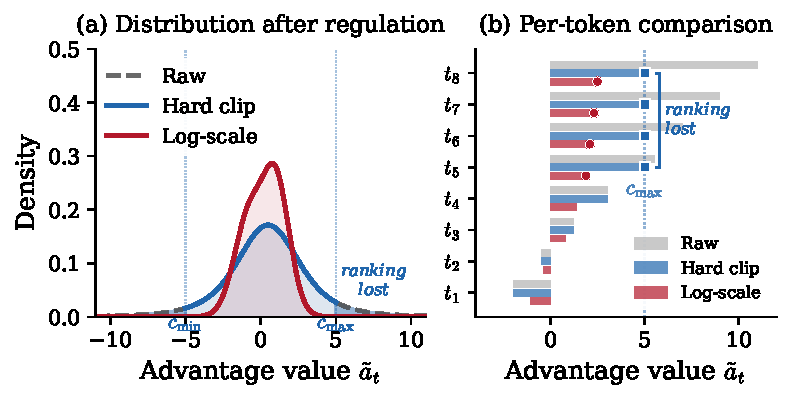
\includegraphics[width=1\linewidth]{figs/signal_regulation_v3.pdf}
%         \caption{Enter Caption}
%         \label{fig:placeholder}
% \end{figure}

\begin{figure}                                                    \centering                         
      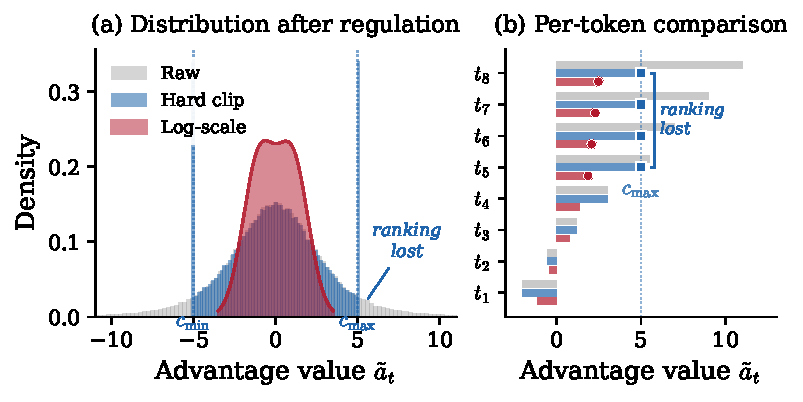
\includegraphics[width=0.95\linewidth]{figs/signal_regulation_v4.pdf}                                   \caption{Hard Clipping collapses all tokens beyond the $[c_{\min}, c_{\max}]$ to the same value (ranking lost). Log-scale compression preserves ordering across the full range.}    
      \label{fig:signal-regulation}   
      \vspace{-3mm}
\end{figure}

% cold start可能会限制student，有policy drift

% \subsection{Stabilizing OPD with Signal Regulation}                

% In the previous section, we identified that naive OPD is prone to training instability: extreme token-level log-ratio values can dominate the policy gradient and trigger length exploitation as shown in Figure~\ref{fig:token-adv}. 
% To address this, we regulate the raw per-token advantage $\Delta\ell_t \triangleq \log\pi_T(y_t)
%    - \log\pi_\theta(y_t)$, preventing outliers from destabilizing training. 
% We consider two variants including Hard Clipping and Soft Compression as the toy illustration shown in  Figure~\ref{fig:signal-regulation}:

%   \begin{itemize}[leftmargin=*]
%         \item \textbf{Clipping.} Hard clipping truncates the advantage to a fixed range:
%     \begin{equation}
%     \label{eq:adv-clip}
%     \tilde{a}_t = \mathrm{clip}\!\bigl(\Delta\ell_t,\; c_{\min},\; c_{\max}\bigr).
%     \end{equation}
%     We set $[c_{\min}, c_{\max}] = [-10, 10]$. Although broad, this range is sufficient to suppress extreme outliers while preserving signal diversity for the majority of tokens.

%     \item \textbf{Log-Scale Compression.} Unlike hard clipping, which silences all signal beyond the bounds, log-scale compression applies a
%   monotonic transformation that preserves the relative ordering of token-level advantages while compressing extreme values:
%     \begin{equation}
%     \label{eq:adv-logscale}
%     \tilde{a}_t = \mathrm{sign}(\Delta\ell_t) \cdot \log\!\bigl(1 + |\Delta\ell_t|\bigr).
%     \end{equation}
%     This retains the teacher's full ranking over tokens without allowing outliers to dominate the gradient.
%   \end{itemize}

% \hongru{any motivation for this log-scale compression? e.g., why log-scale compression? an other compression?}

\subsection{Stabilizing OPD with Signal Regulation}        
\label{sec:regulation}


Motivated by the aforementioned pathologies, we transition from diagnosing length exploitation to developing proactive in-loop remedies. 
To prevent extreme token-level log-ratios from dominating the policy gradient, which \textbf{exacerbates the teacher–student mismatch and enables the student to exploit length through extreme signals}, we introduce token-level signal regulation.

Our design follows two principles: \textbf{(1) Preference preservation}, regulation must not reverse the teacher's ordinal signal; \textbf{(2) Outlier suppression}, pathologically large magnitudes should be dampened without discarding fine-grained token-level information.
We investigate two complementary paradigms, representing \emph{Hard truncation} and \emph{Soft compression} respectively (Figure~\ref{fig:signal-regulation}):

% To prevent extreme token-level log-ratios from dominating the policy gradient and triggering length exploitation, we introduce token-level signal regulation. We investigate two complementary paradigms—representing \emph{hard truncation} and \emph{soft compression} respectively (Figure~\ref{fig:signal-regulation})—to process the raw advantage $\Delta\ell_t \triangleq \log\pi_T(y_t|y_{<t}) - \log\pi_\theta(y_t|y_{<t})$:

\begin{itemize}[leftmargin=*,nosep]
    \item \textbf{Hard Clipping.} As a representative of rigid thresholding, this method truncates the advantage into a deterministic bound to eliminate severe outliers while preserving signal diversity:
    \begin{equation}
    \small
    \label{eq:adv-clip}
    \tilde{\Delta\ell}_t = \mathrm{clip}\!\bigl(\Delta\ell_t,\; c_{\min},\; c_{\max}\bigr).
    \end{equation}
    % We set $[c_{\min}, c_{\max}] = [-10, 10]$ to eliminate severe outliers while preserving signal diversity for other tokens.

    \item \textbf{Soft Log-Scale Compression.} As a smooth alternative, this method dampens unbounded signals without discarding the relative rankings beyond fixed bounds:
    \begin{equation}
    \label{eq:adv-logscale}
    \small
    \tilde{\Delta\ell}_t = \mathrm{sign}(\Delta\ell_t) \cdot \log\!\bigl(1 + |\Delta\ell_t|\bigr).
    \end{equation}
    The choice of $\log(1+|x|)$ is motivated by its dual-regime properties. Near zero, it approximates a linear mapping ($\tilde{\Delta\ell}_t \approx \Delta\ell_t$), fully preserving the teacher's fine-grained preferences. Crucially, when $|\Delta\ell_t| \to \infty$, its sub-linear growth radically compresses the magnitude of unbounded values. 
    % This scaling contract ensures that pathological outliers are tightly bound, preventing them from destabilizing the policy gradient updates and dominating the optimization loop.
\end{itemize}

% \vspace{-0.1mm}
\paragraph{Experiment Setup} 
To explore the performance of the above two optimization techniques for OPD, we utilize Qwen3-1.7B-GRPO, Qwen3-4B-GRPO as the teachers, and Qwen3-1.7B-Base and Qwen3-1.7B as the students. 
For better comparison, we select current OPD variants as counterparts~\cite{eopd,gopd,hou2026uni}.
The performance of Qwen3-1.7B-Base as the student is shown in Table~\ref{tab:main}, and the scores of Qwen3-1.7B are shown in Table~\ref{tab:unified_math_results}.



\begin{figure}
    \centering
    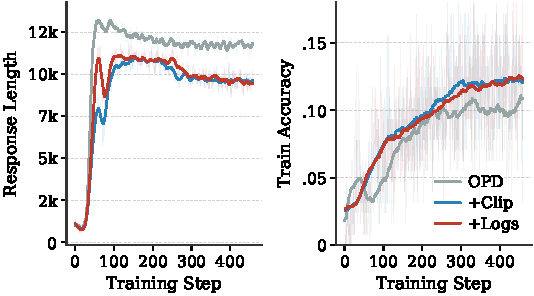
\includegraphics[width=\linewidth]{figs/three-runs-compare.pdf}
    \caption{Training dynamics of OPD variants. Teacher: Qwen3-4B-GRPO; Student: Qwen3-1.7B-Base. Vanilla OPD suffers greater 
  length exploitation, whereas Clip produces \textbf{shorter responses and achieves higher accuracy} than naive OPD.}
    \label{fig:dya-from-4b}
    \vspace{-3mm}
\end{figure}

\subsection{Analysis}

\paragraph{Signal Regulation is Effective.}
As shown in Table~\ref{tab:main}, both regulation variants yield clear improvements over naive OPD.
With the 1.7B-GRPO teacher, OPD+Clip brings substantial gains across all benchmarks.
Comparing the two variants, log-scale compression outperforms hard clipping for Qwen3-1.7B-Base, likely because it retains the teacher's full token ranking rather than flattening extreme values to the clip boundary.

\noindent \textbf{Alleviating the Student-Teacher Mismatch.}\quad
Our experiments further demonstrate that {naively scaling up the teacher does not guarantee better student performance}. 
Hard clipping partially rescues this, lifting the 4B-guided student back to 28.1 of average score. 
Interestingly, log-scale compression, which excelled with the 1.7B teacher, fails to yield comparable gains here, as the training dynamics shown in Figure~\ref{fig:dya-from-4b}. 
We attribute this to the nature of the distributional shift: a much stronger teacher heavily mixes genuine correctness cues with biases in its advantages. 
Log-scale compression preserves this noise, whereas hard clipping aggressively truncates it. 
This yields a crucial insight: \textbf{when the teacher-student gap is large, aggressively truncating extreme signals is more effective than compressing them.}

\paragraph{Impact of Student Capacity}
% Comparing Tables~\ref{tab:main} and~\ref{tab:unified_math_results} reveals a striking interaction between student capacity and teacher strength. 
% When the student is upgraded from a base model to the post-trained {Qwen3-1.7B}, the mismatch alleviates.
% The 4B-GRPO teacher now delivers the best results, decisively outperforming the 1.7B-GRPO teacher. This confirms that the trap stems from the distributional mismatch with a \emph{weak} student, not solely the teacher's absolute strength. 
% Demonstrating that proper teacher and student selection, with signal regulation, could effectively surpass those counterparts with much larger and stronger teachers. 

% \paragraph{Student Capacity Dictates Distillation Ceilings.}
Comparing Tables~\ref{tab:main} and~\ref{tab:unified_math_results} reveals a striking impact between student capacity and teacher strength. 
When the student is upgraded from a base model to the post-trained {Qwen3-1.7B}, the initial distributional mismatch is significantly mitigated. 
{Consequently, the performance hierarchy flips:} {Qwen3-4B-GRPO} teacher now delivers the best results, decisively outperforming the {Qwen3-1.7B-GRPO} teacher. 
This shift confirms that the trap stems from the capability gap with student-teacher mismatch. 
{Crucially, by resolving this mismatch,} our regulated OPD with a 4B teacher ultimately surpasses previous methods distilled from a larger 30B teacher. 
This demonstrates that proper capacity matching combined with signal regulation can eclipse brute-force parameter scaling.

\section{Related Work}

\paragraph{On-Policy Distillation.}
\begin{table}[t]
    \small
    \centering
    \setlength{\tabcolsep}{5pt} % 紧凑间距，确保在 ACL 双栏排版中完美契合单栏宽度
    \renewcommand{\arraystretch}{1.2}
    \begin{tabular}{l cccc}
    \toprule
    \textbf{Method} & \textbf{AIME24} & \textbf{AIME25} & \textbf{AIME26} & \textbf{HMMT25} \\
    \midrule
    
    % --- 第一组 ---
    \rowcolor{gray!10} \multicolumn{5}{c}{\textit{\textbf{Teacher: Qwen3-30B-A3B-Instruct-2507}}} \\
    \rowcolor{gray!10} Teacher     & 74.7 & 62.8 & 63.3 & 44.2 \\
    \textbf{UniOPD}      & 35.2 & 30.7 & --   & 17.7 \\
    \textbf{GOPD}       & 37.3 & 31.5 & --   & 16.2 \\
    
    \midrule 
    % --- 第二组 ---
    \rowcolor{gray!10} \multicolumn{5}{c}{\textit{\textbf{Teacher: Qwen3-1.7B-GRPO}}} \\
    \rowcolor{gray!10} Teacher     & 41.9 & 32.5 & 37.5 & 21.7 \\
    \textbf{CLIP}        & \underline{44.4} & \underline{32.5} & \underline{35.9} & \textbf{20.9} \\
    
    \midrule
    % --- 第三组 ---
    \rowcolor{gray!10} \multicolumn{5}{c}{\textit{\textbf{Teacher: Qwen3-4B-GRPO}}} \\
    \rowcolor{gray!10} Teacher     & 64.4 & 57.1 & 57.3 & 37.3 \\
    \textbf{CLIP}        & \textbf{45.2} & \textbf{37.5} & \textbf{36.0} & \underline{19.0} \\
    \bottomrule
    \end{tabular}
    \caption{Performance of Qwen3-1.7B student tuned by OPD+Clip (CLIP) and previous methods~\cite{hou2026uni,gopd}, which further proves that \textit{a stronger teacher cannot ensure better student performance}. The \textbf{best} and the \underline{second best} scores are marked.  }
    \label{tab:unified_math_results}
    \vspace{-3mm}
\end{table}

% \hongru{above is lengthy.}
Early formulations of OPD optimized a reverse-KL objective to restrict the student to the teacher's high-probability modes~\citep{gu2026minillmonpolicydistillationlarge,GKD2024}. Subsequent work reframed the teacher's per-token log-ratios as dense rewards capable of shaping exploration trajectories~\citep{gopd}, fueling its rapid adoption in scale post-training~\citep{deepseekai2026deepseekv4,qwen3,glm5team2026glm5vibecodingagentic,Nemotron-Cascade-2}.
Despite this widespread use, the failure conditions of this dense guidance remain poorly understood. 
Prior exploratory studies attribute training instability to factors like thinking-pattern compatibility, offering external fixes such as prompt alignment or cold-start initialization~\cite{li2026rethinkingonpolicydistillationlarge,opd-var-1,yu2026dopddualonpolicydistillation}. 
% In contrast, we look inside the black box to analyze the fidelity of token-level advantages directly. We show that stability depends less on external teacher alignment and more on preventing the optimization objective from degenerating into length exploitation and distribution mismatch.
Our work takes a fundamentally parallel yet deeper trajectory: we diagnose signal-level pathologies (student-teacher mismatch and length exploitation) and propose zero-overhead in-loop regulations (clipping and log-scale compression) that require neither off-policy data nor prompt filtering.




% \paragraph{Capacity Gap in Knowledge Distillation.}
% A recurring finding in KD is that excessively capable teachers can degrade student performance.
% \citet{cho2019efficacy} first demonstrated that distillation can hurt when the teacher is substantially more capable, and \citet{mirzadeh2020improved} proposed teacher assistants to bridge the gap.
% \citet{busbridge2025distillation} quantify this via distillation scaling laws, identifying a U-shaped regime where teacher over-capability hurts efficiency.
% For LLM reasoning, \citet{li2025learnability} shows that long chain-of-thought traces from strong teachers consistently underperform simpler approaches for small students.

% Our work extends this line to the on-policy setting, providing a signal-level explanation for why stronger teachers fail, and proposing in-loop regulation rather than architectural changes.

\paragraph{Capacity Gap in Knowledge Distillation.}
% A recurring phenomenon in knowledge distillation (KD) is that excessively capable teachers can unexpectedly degrade student performance. 
% \citet{cho2019efficacy} found that the higher teachers' accuracies on benchmarks do not necessarily mean better teachers.
% \citet{li2026rolereasoningpatternsgeneralization} found that the thinking patterns of teachers and students impact distillation performance
% \citet{kd-from-strong-1} found that the prediction discrepancy between the teacher and the student is severe, and utilizing the rec label preference order of the teacher to alleviate this.
% \citet{mirzadeh2020improved} proposed using intermediate teacher assistants to bridge the rift. 
% Within the context of LLM reasoning, this learnability barrier is equally pronounced.
% \citet{li2025learnability} observed that complex, long reasoning traces generated by strong teachers consistently underperform simpler, teacher-free approaches when distilled into smaller student models.

A recurring phenomenon in knowledge distillation (KD) is that excessively capable teachers can unexpectedly degrade student performance. Specifically, \citet{cho2019efficacy} noted that higher benchmark accuracy in teachers does not inherently translate into superior distillation efficacy.  To mitigate the structural mismatches between models, various strategies have been proposed: \citet{kd-from-strong-1} identified a severe prediction discrepancy between teachers and students, proposing the utilization of the teacher's recommendation label preference order to alleviate the gap, while \citet{mirzadeh2020improved} introduced intermediate teacher assistants to bridge this capacity rift.
Within the context of reasoning, this learnability barrier remains equally pronounced. For instance, \citet{li2025learnability} observed that complex, long reasoning traces generated by strong teachers consistently underperform simpler, teacher-free approaches when distilled into smaller student models. \citet{li2026rolereasoningpatternsgeneralization} demonstrated that the alignment of thinking patterns between teachers and students profoundly impacts distillation outcomes.

Our work extends this classic line of inquiry into the on-policy regime.  Rather than merely documenting the empirical decay caused by strong teachers, we offer a precise, signal-level explanation for \emph{why} and \emph{when} these advanced guidance signals corrupt on student-generated rollouts. Furthermore, we demonstrate that the capability gap can be mitigated via lightweight, in-loop signal regulation.

% \section{Conclusion}
% We presented a systematic study of on-policy distillation through three lenses.
% We first established that OPD acts as an \emph{exploration catalyst} whose benefit scales with problem diversity, not rollout depth.
% We then diagnosed two pathologies: the \emph{Strong Teacher Trap} (negative informativeness from distributional mismatch) and \emph{Length Exploitation} (token-level shortcuts at both length extremes).
% Finally, we showed that lightweight signal regulations, hard clipping, and log-scale compression eliminate these failures without additional compute, enabling a 4B teacher to surpass methods using larger teachers.
% Our central takeaway is that \textit{signal quality, not teacher scale, governs OPD success}.
\section{Conclusion}
\label{sec:conclusion}

In this work, we look inside OPD to shift the paradigm from empirical scaling to rigorous signal-level diagnosis. 
We first established that OPD acts as an \emph{exploration catalyst} which benefits more from problem diversity.
Then we systematically expose two critical pathologies: \emph{length exploitation} via redundant token padding, and the \emph{Student-Teacher Mismatch}, where severe capabilities mismatch causes negative impacts. 
To restore guidance fidelity, we introduce lightweight signal regulations that require zero off-policy overhead. Our empirical results demonstrate that regulating token-level advantage dynamics effectively eliminates these failures, enabling a 4B teacher to surpass configurations distilled from larger models,  which is \textit{signal quality, not teacher scale, governs OPD success}.

% \clearpage

\section*{Limitations}
Although our proposed hard clipping and soft log-scale compression strategies effectively restore guidance fidelity and stabilize training, they introduce hyperparameter heuristics that require empirical tuning based on the specific teacher-student capacity gap. A dynamic, adaptive regulation framework could be further explored.
Our systematic empirical study primarily focuses on mathematical reasoning benchmarks, where outcomes are easily verifiable and reasoning chains are dense. 
The behavior of regulated OPD in open-ended text generation or knowledge-intensive QA tasks has not been fully verified.

\bibliography{custom}

\appendix

\section{Experiment Configurations}
We implement the training pipeline using {verl}.
For the OPD pipeline, policy optimization uses a total batch size of $128$, 1 rollout for each prompt. 
For the GRPO baselines, the group advantage is calculated across a size of $128 \times 8$ rollouts. Optimization is limited to a single epoch per rollout batch to eliminate off-policy bias.
The maximum sequence length is set to $16,384$ tokens during training. 
Rollouts are generated using stochastic sampling with a temperature of $\tau = 1.0$ and $\text{top-}p = 1.0$.

For the avg@32 metric, we utilized $N=40$ candidate responses per problem for better estimation. To obtain a stable estimation, we perform $M=10$ independent trials. In each trial, we randomly sample a subset of $k=32$ responses from the candidate pool and calculate the correctness of the $j$-th response as $\mathbb{I}_j \in \{0, 1\}$. The final score is the average across all trials, formulated as:
\begin{equation}
\text{avg@}32 = \frac{1}{M} \sum_{i=1}^{M} \left( \frac{1}{k} \sum_{j \in \mathcal{S}_i} \mathbb{I}_j \right)
\end{equation}

% Our complete training code and experimental configuration files will be made publicly available upon publication.

\end{document}
